\documentclass{bredelebeamer}
\usepackage{caption}
\usepackage{graphicx}
\usepackage{subcaption}
\usepackage{tabulary}
\usepackage{bm}
\usepackage{algpseudocode}
\usepackage[textwidth=8em,textsize=small]{todonotes}
\usepackage{amsmath,mathtools,bbm}
\usepackage{amsthm}

\usepackage{algorithm}

\graphicspath{ {Images/} }


%%%%%%%%%%%%%%%%%%%%%%%%%%%%%%%%%%%%%%%%%%%%%%%%



\title[Stats for Bio]{Introduction to Statistics and Machine Learning}
% Titre du diaporama

% Sous-titre optionnel

\author{Oliver M. Crook}
% La commande \inst{...} Permet d'afficher l' affiliation de l'intervenant.
% Si il y a plusieurs intervenants: Marcel Dupont\inst{1}, Roger Durand\inst{2}
% Il suffit alors d'ajouter un autre institut sur le modèle ci-dessous.

\institute[University of Cambridge]
{
  \inst{ }%
  DAMTP, Department of Biochemistry, MRC Biostatistics Unit\\
  University of Cambridge
}	


\date{23 July 2019}
% Optionnel. La date, généralement celle du jour de la conférence

\subject{Sujet de votre diaporama}
% C'est utilisé dans les métadonnes du PDF



%%%%%%%%%%%%%%%%%%%%%%%%%%%%%%%%%%%%%%%%%%%%%%%%%%%%%%%%%%%%%%%%%%%%%
\begin{document}

\begin{frame}
  \titlepage
\end{frame}





\begin{frame}{Summary}
  \tableofcontents
  % possibilité d'ajouter l'option [pausesections]
\end{frame}




\section{Introduction}

\begin{frame}{What is statistics/machine learning?}
\begin{itemize}
\item Learn from data
\item Draw inference from data to make scientific conclusions
\item Test scientific hypothesis quantitatively
\item Make sound predictions
\item Visualising raw data, visualise processed data and visualise conclusions 
\end{itemize}
\end{frame}

\begin{frame}{Visualisation, visualisation, visualisation}
	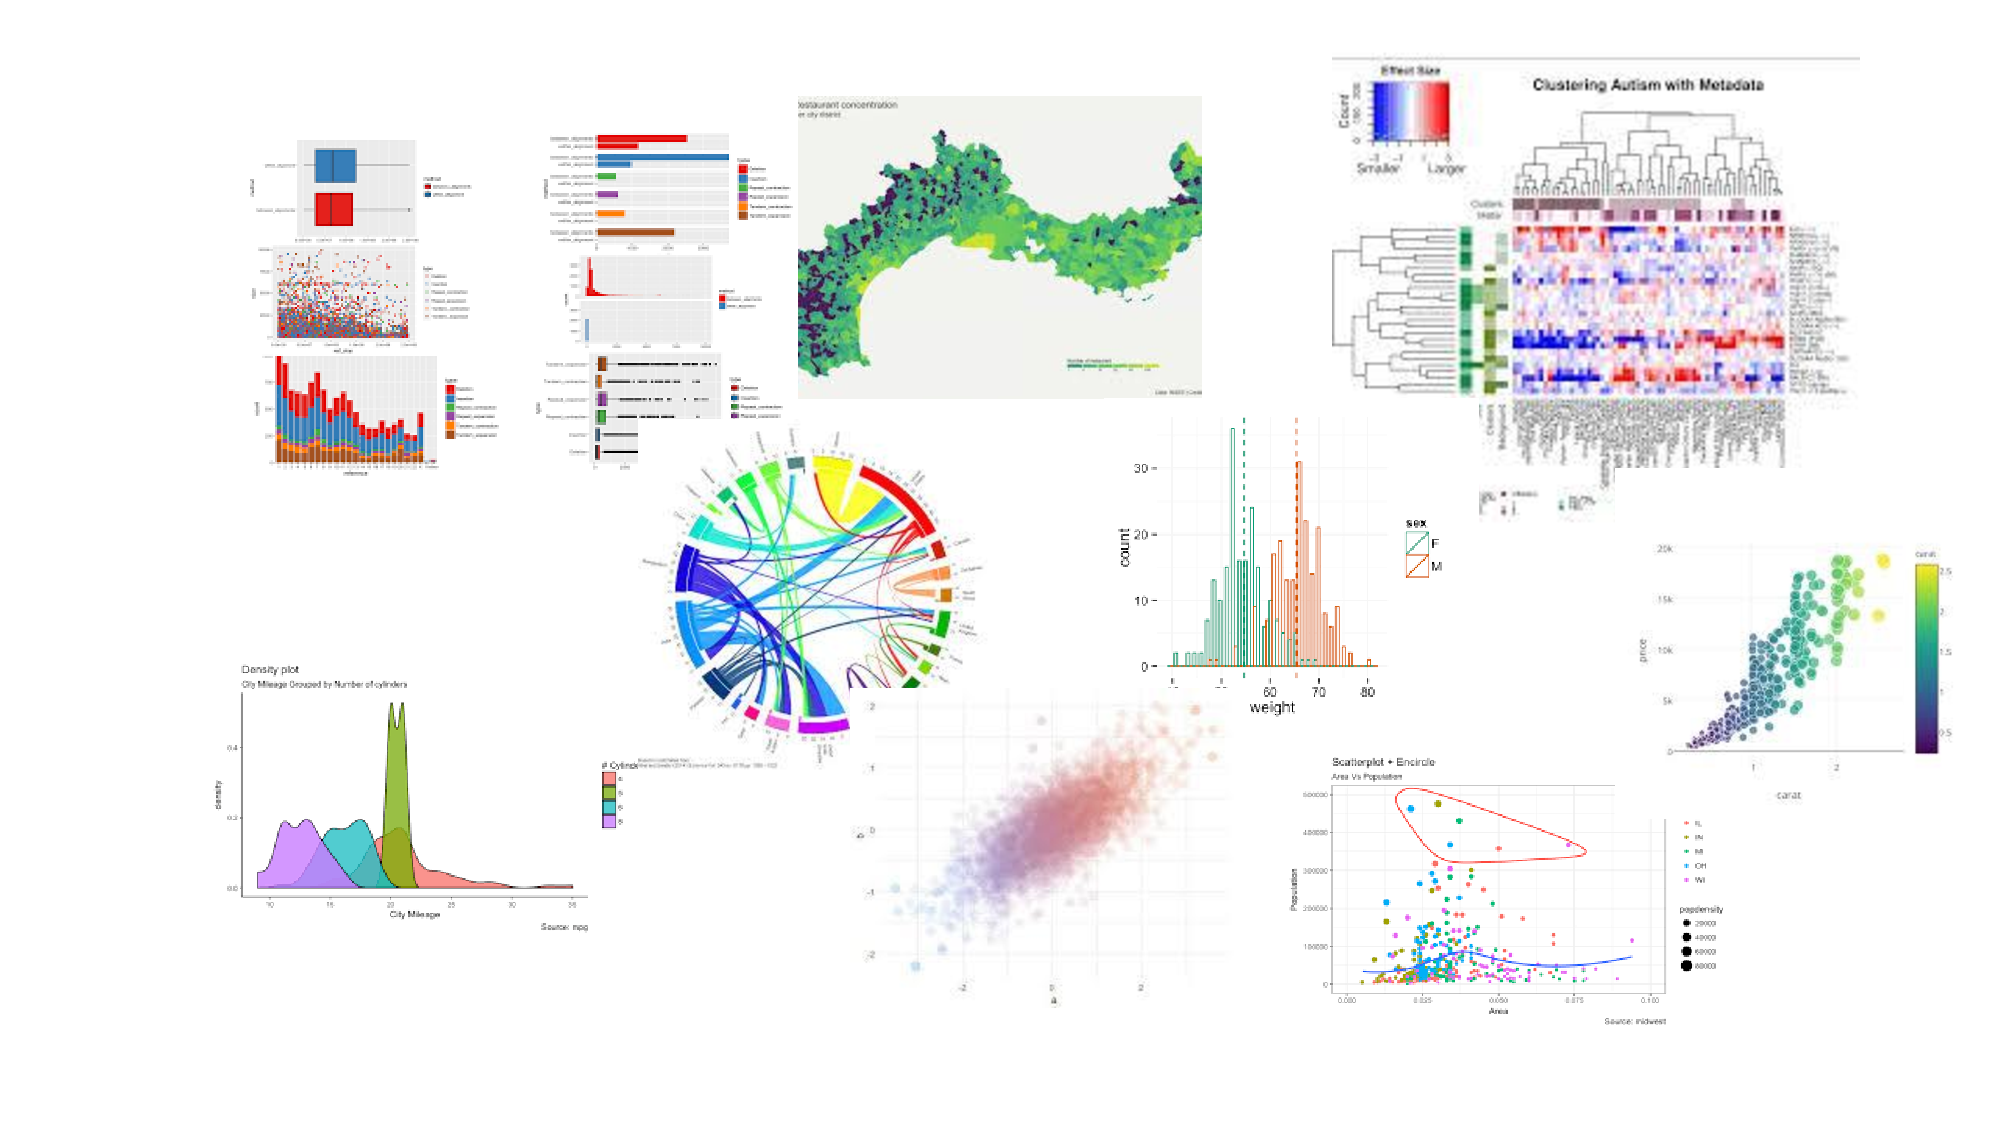
\includegraphics[width=1\textwidth]{visualise.pdf}
\end{frame}

\section{Hypothesis Testing}
\begin{frame}{What does a hypothesis test aim to do?}
\begin{block}{Hypothesis Testing}
	\begin{itemize}
	\item We want to draw conclusions or make decisions based on data.
	\item Screening of potentially millions of possible avenues to follow up.
	\item Example genome-wide association studies test millions of variants.
	\item Infeasible to looks at every variant functionally.
	\item Only follow up variants that statistics "recommends". 
	\end{itemize}  
\end{block}
\end{frame}

\begin{frame}{Example: Is my coin biased?}
 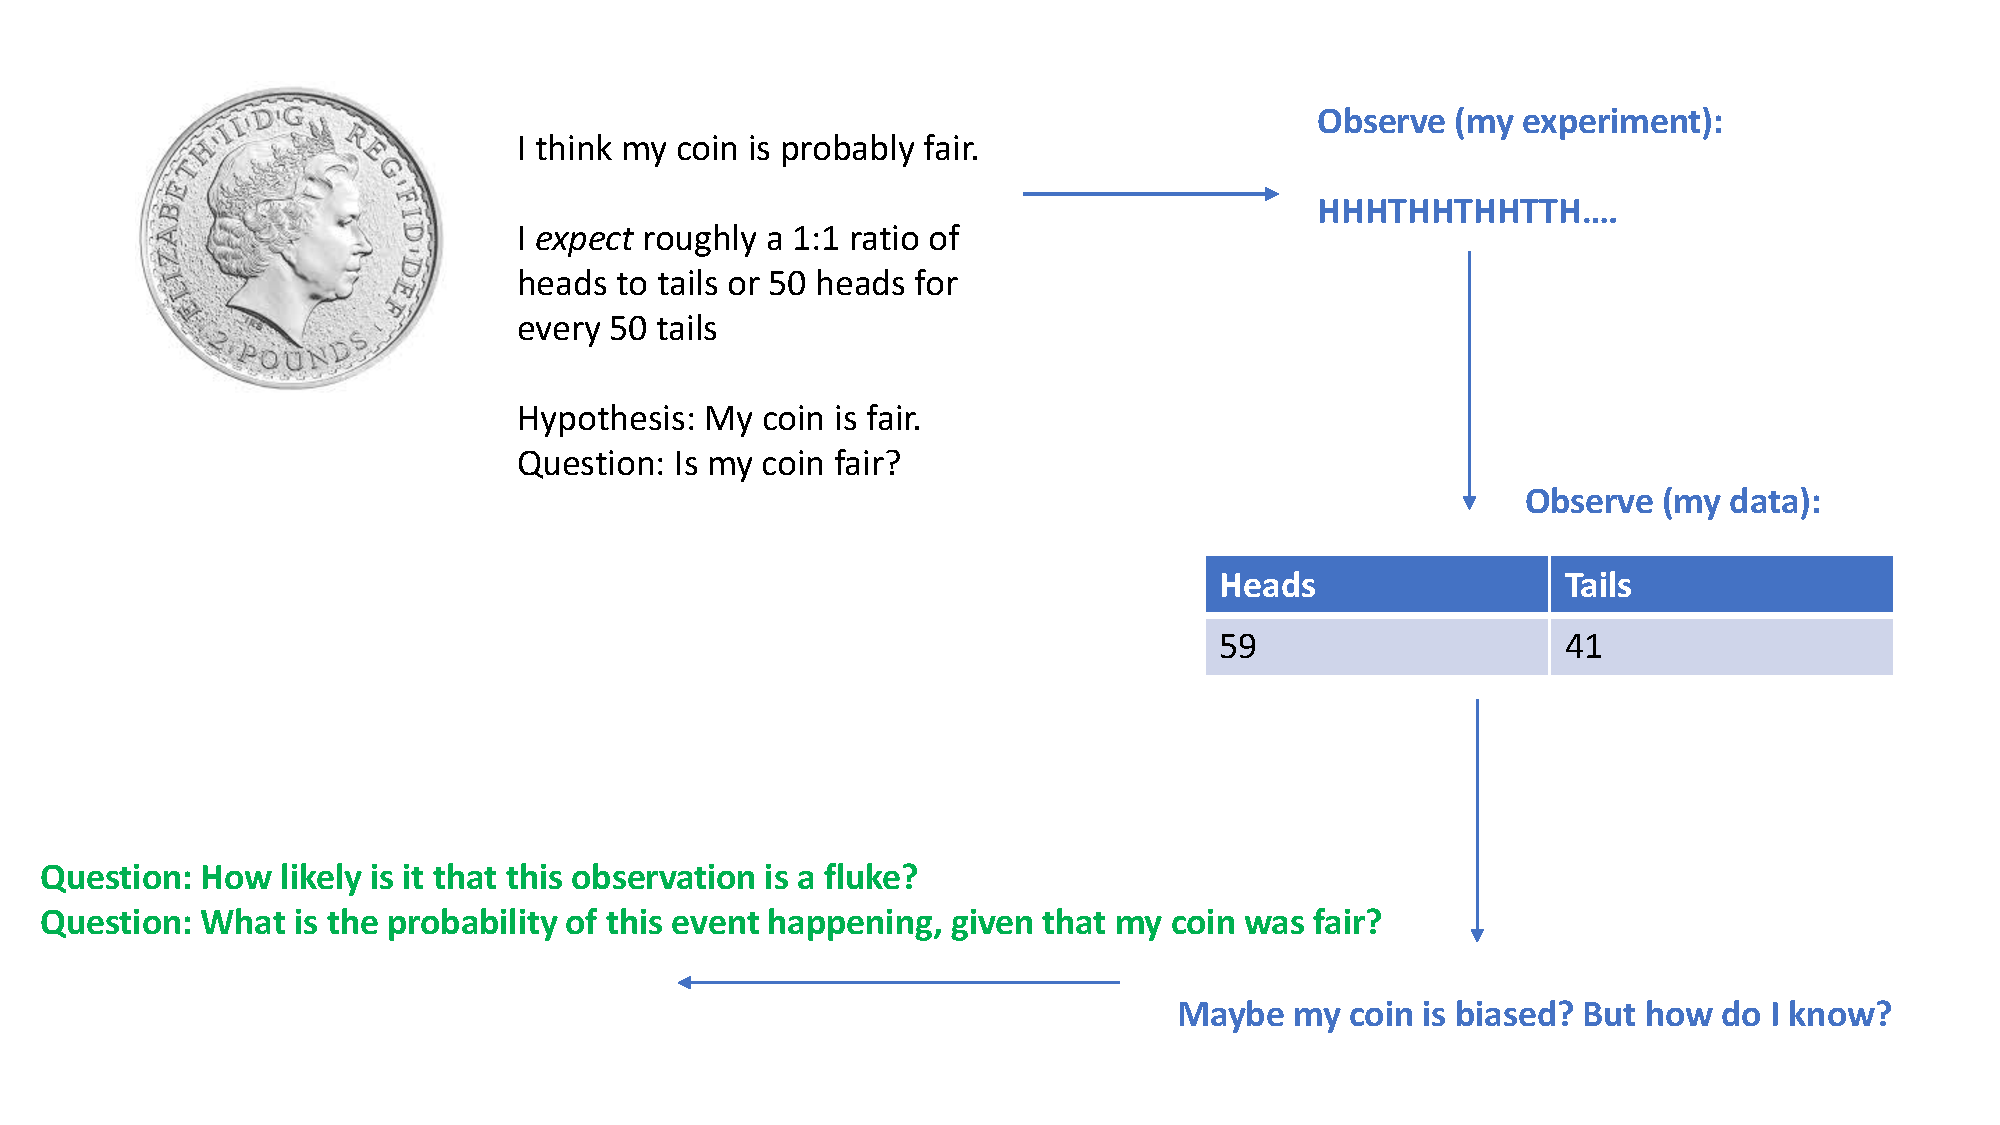
\includegraphics[width=1\textwidth]{cointoss.pdf}
\end{frame}

\begin{frame}{First observations}
\begin{block}{Observations}
	\begin{itemize}
		\item Statistics started before we did any experiments
		\item We made some statements before any experimentation
		\item We formed a hypothesis (which we call the null hypothesis)
		\item We designed an experiment and observed data
		\item We asked a clear statistical question
	\end{itemize}
\end{block}
\end{frame}

\begin{frame}{...yes, but is my coin biased?}
Our test statistic
\begin{equation}
P(K = k|n, p) = {n \choose k}p^k(1-p)^{n - k}
\end{equation}
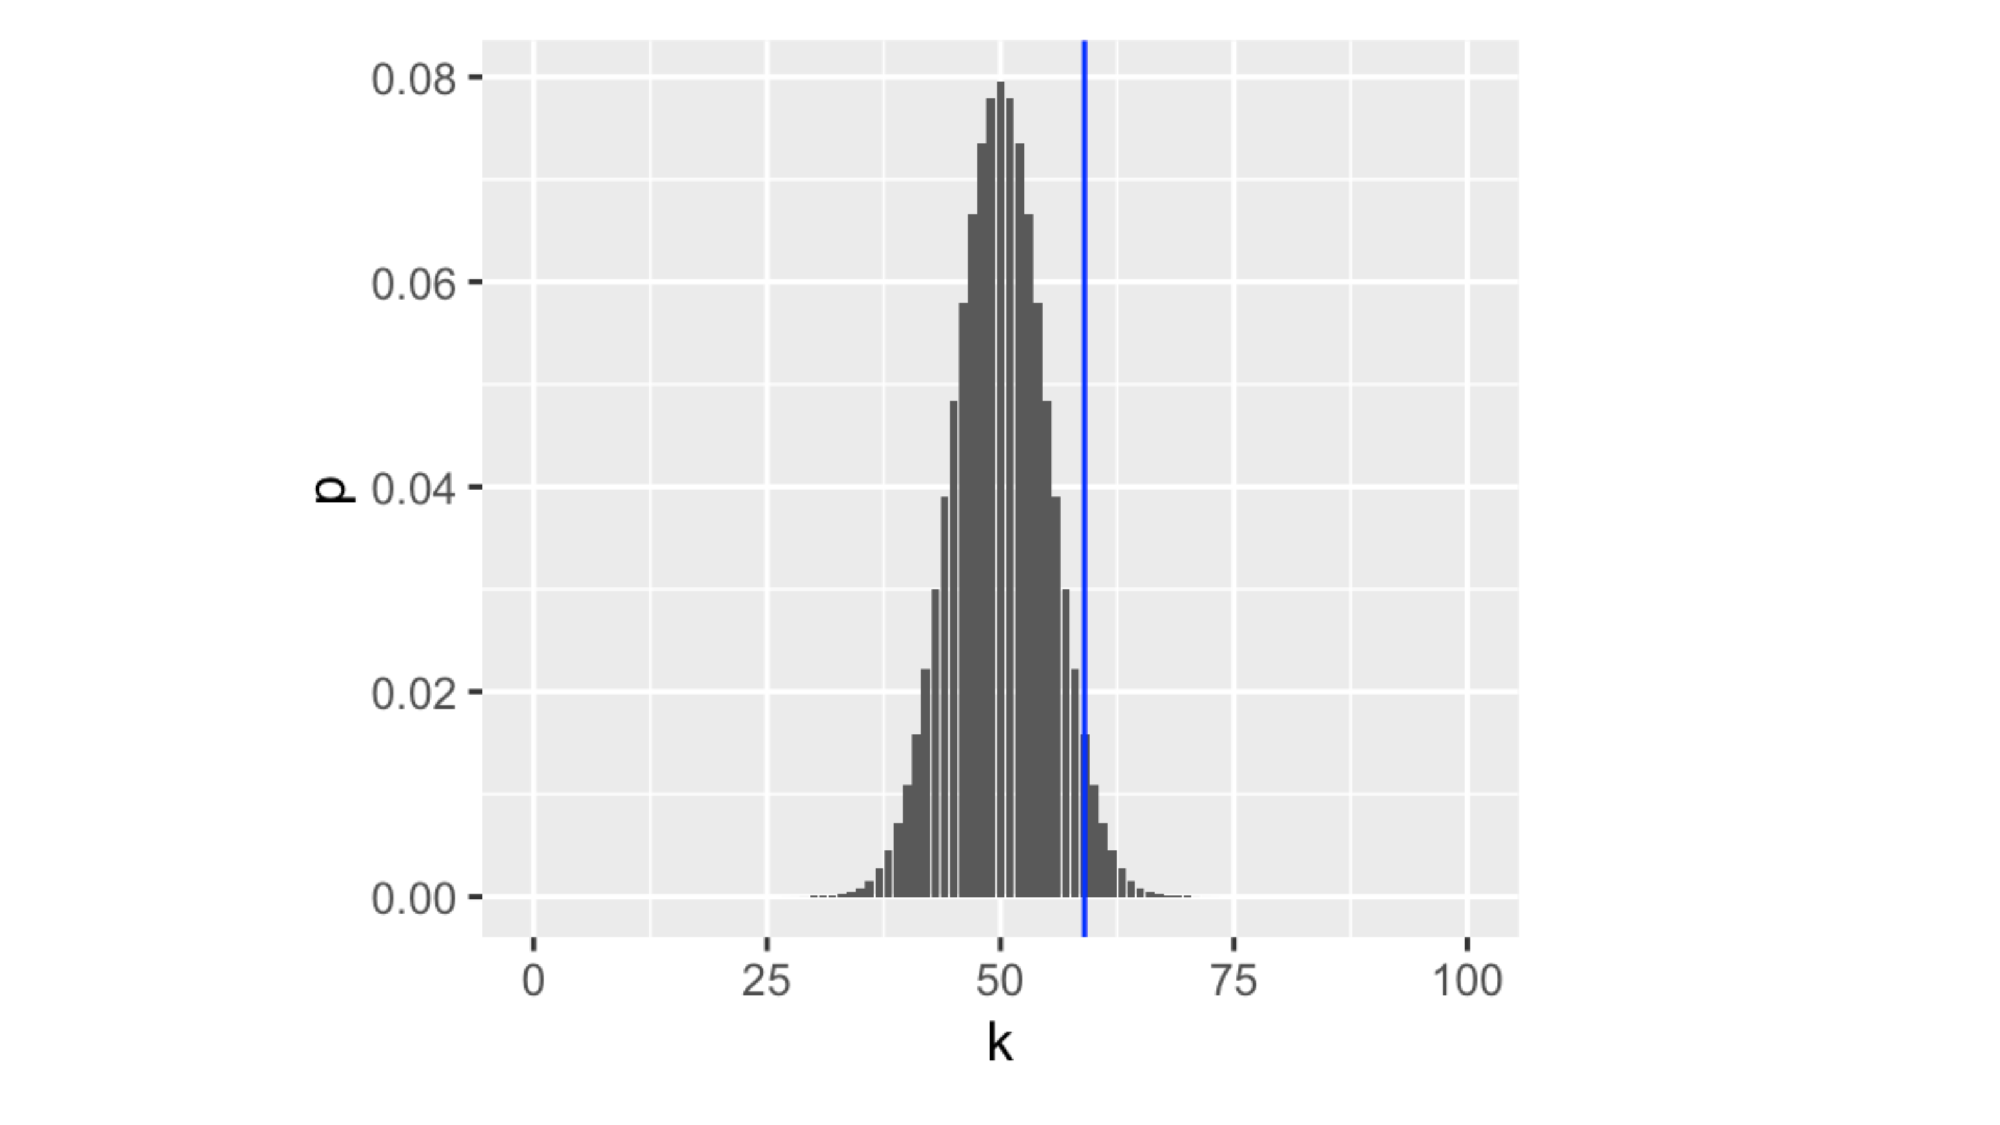
\includegraphics[width=1\textwidth]{teststatistics}



\end{frame}

\begin{frame}{...yes, but is my coin biased?}
\begin{block}{Observations}
	\begin{itemize}
		\item The blue line seems unlikely (it is in a region of low probability)
		\item What do I need to do to concluded the coin is biased?
		\item Form a region, called the reject region.
		\item Fill the reject region with as many possible values of $k$ such that total probability is less than $0.05$.
		\item These events are unlikely by definition (they have probability less than $0.05$)
	\end{itemize}

\end{block}

\end{frame}

\begin{frame}{the reject region}
(Explicit example in practical)
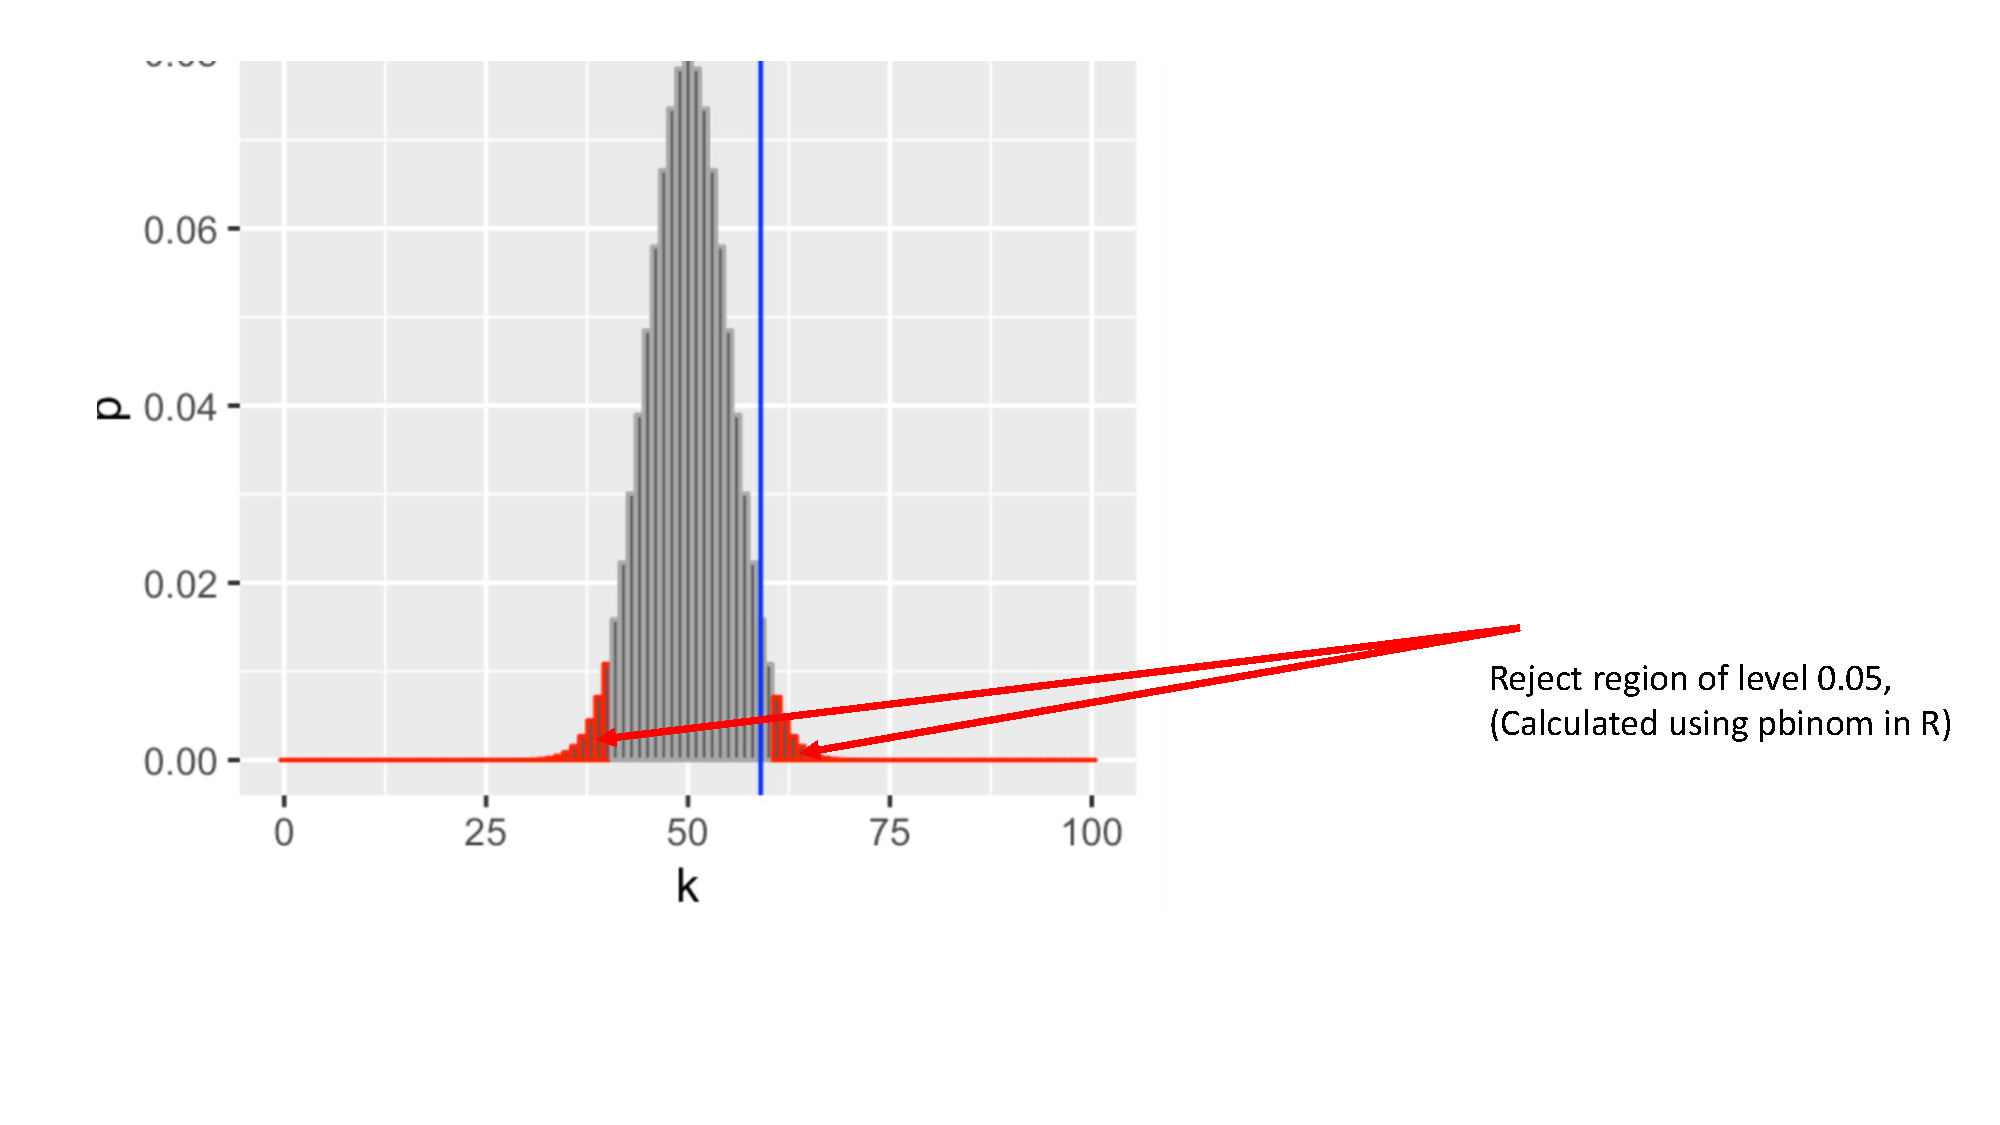
\includegraphics[width=1\textwidth]{rejectregion}
The blue line does not fall in the reject region. We do not reject the hypothesis that the coin is fair. If we saw 75, say, heads we would have rejected the hypothesis that the coin is fair.
\end{frame}


\begin{frame}{The steps to hypothesis test success }
\begin{block}{The hypothesis test journey}
	
	\begin{itemize}
		\item Decide on a quantity you are interested in.
		
		\item Design a suitable experiment.
		
		\item Choose a data summary. 
		
		\item Decide on a test statistic.
		
		\item Set up a simple null hypothesis. (You need to be able to do computations)
		
		\item Decide on the rejection region.
		
		\item Do the experiment and collect the data.
		
		\item Compute the test statistic.
		
		\item Make a decision.
	\end{itemize}

\end{block}
\end{frame}

\begin{frame}
\begin{block}{Definition, Definition, definition}
	
	\begin{itemize}
		\item Significance level or false positive rate $\alpha$: is the total probability of the test statistic falling into this region even if the null hypothesis is true.
		
		\item We now its size, but what's it shape?
		
		\item  We want the rejection region to be as large possible if the alternative hypothesis is true.
		
		\item We want high power (or true positive rate).
	\end{itemize}
	
\end{block}

\end{frame}

\begin{frame}{The null and the alternative}
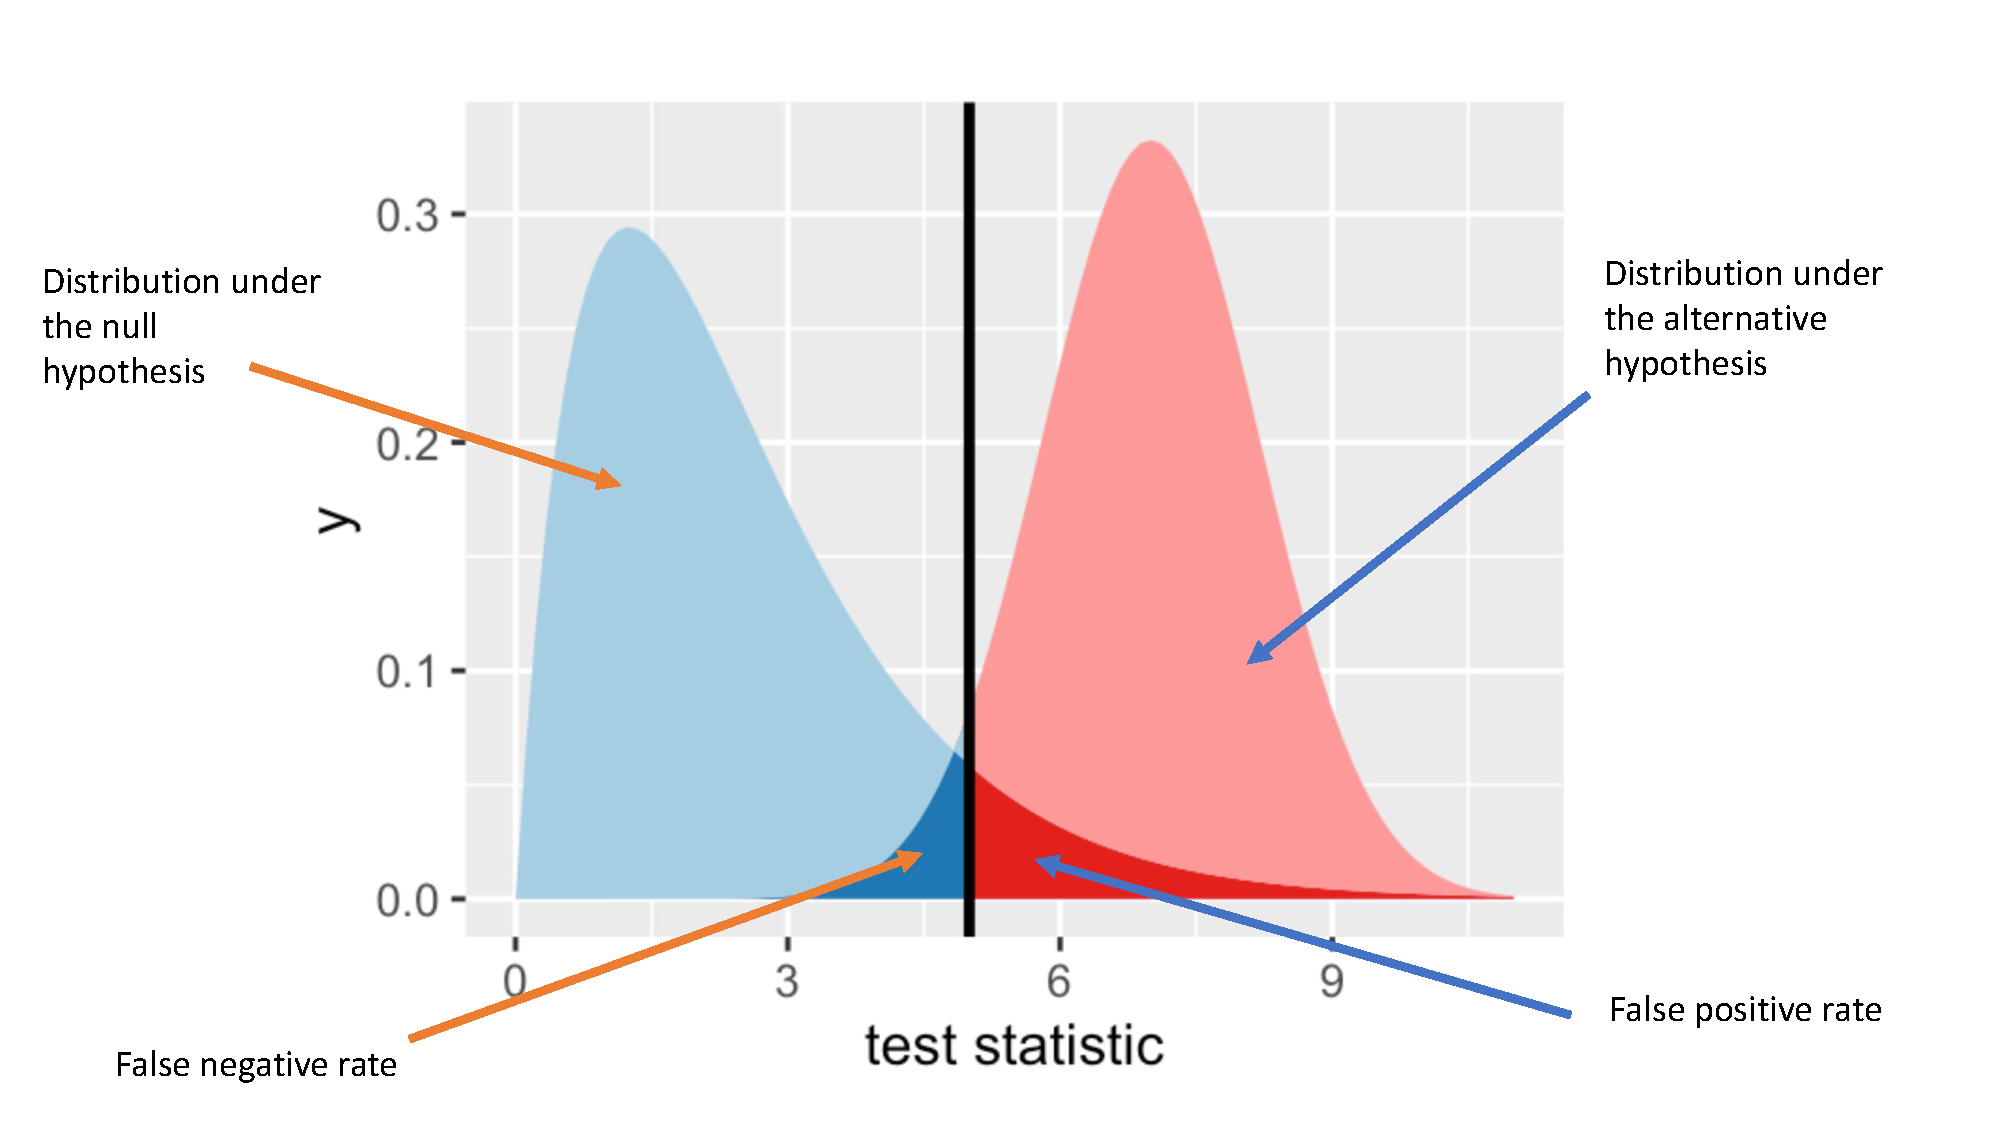
\includegraphics[width=1\textwidth]{nullalt}
\end{frame}

\begin{frame}{Types of Errors}

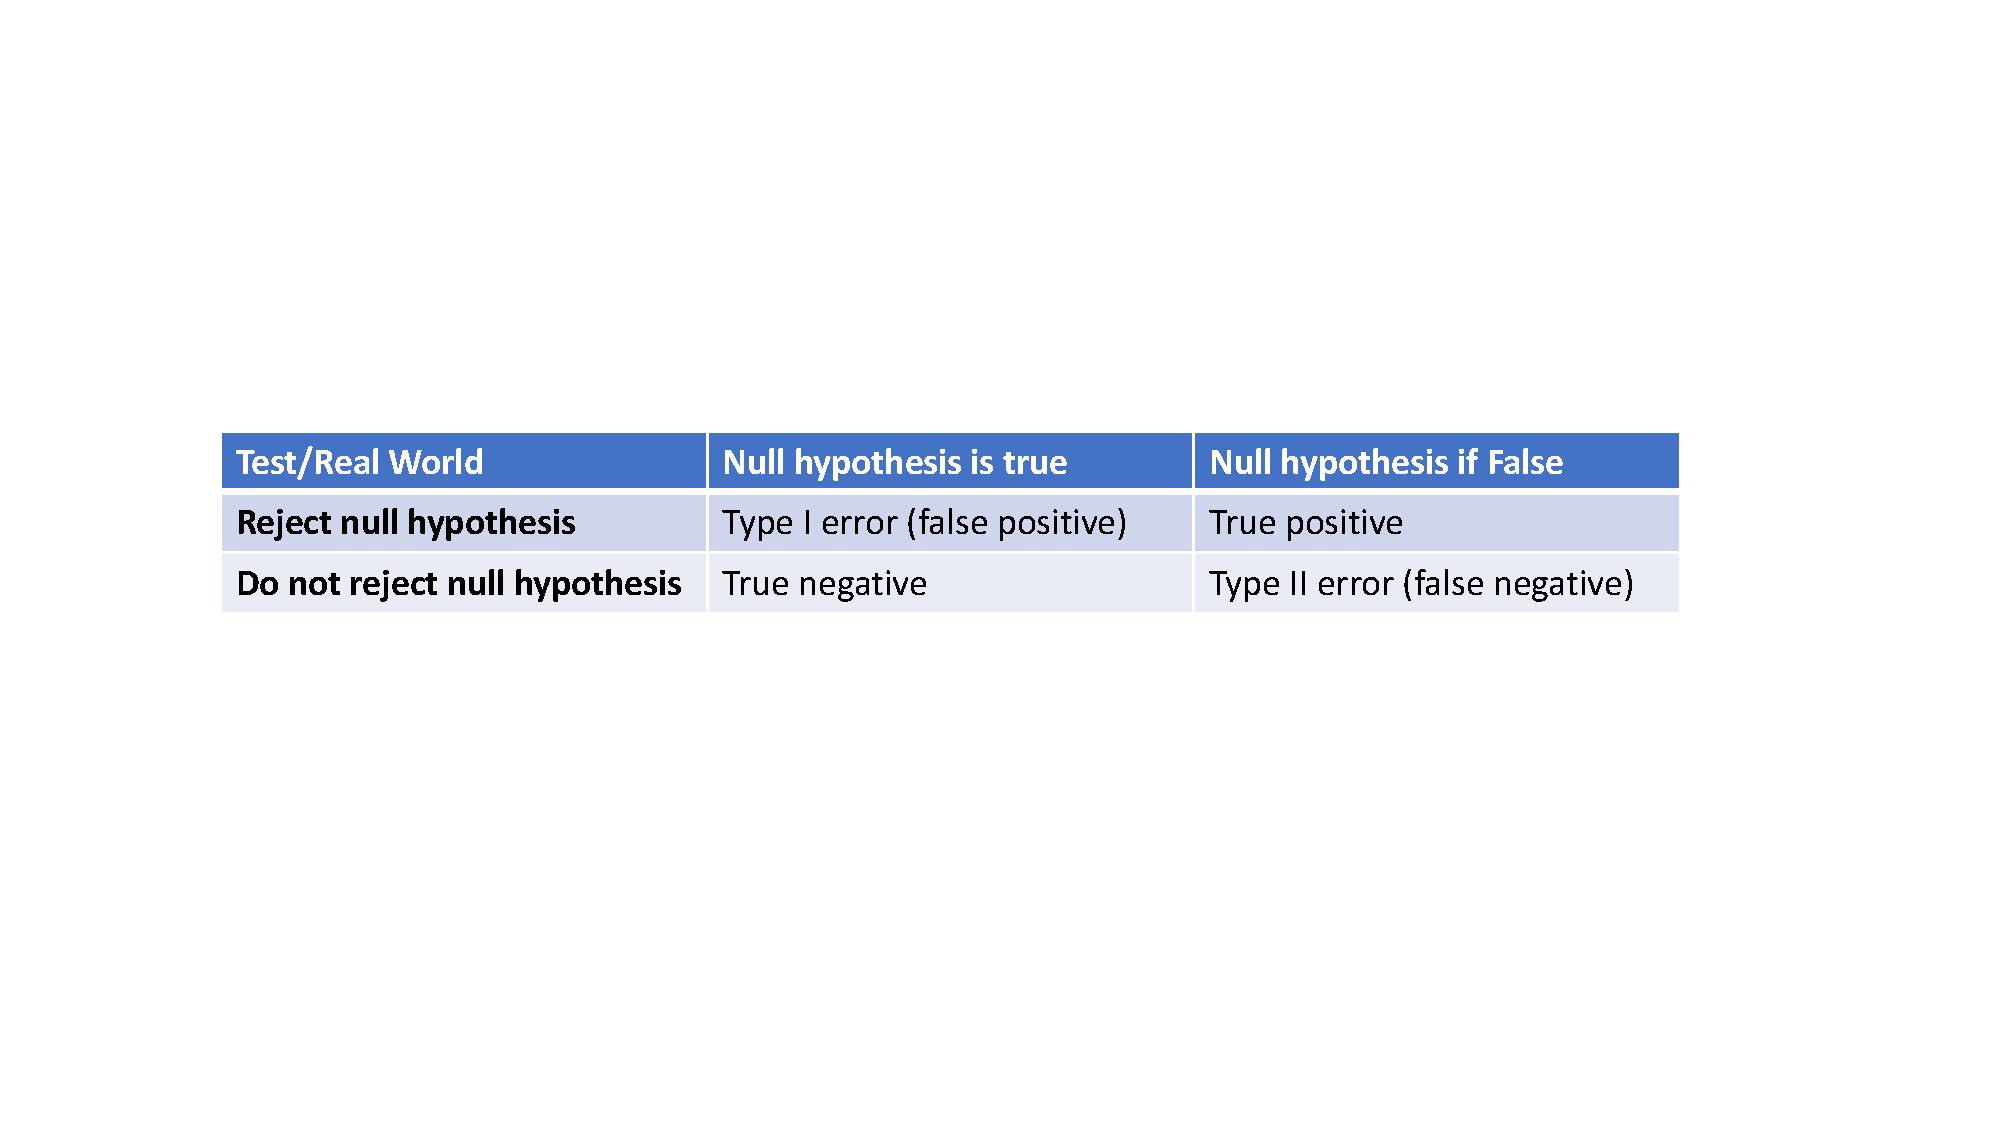
\includegraphics[width=1.2\textwidth]{typeerrors}

\end{frame}

\begin{frame}{Difference between groups: The t-test}
Imagine the following scenario:
\begin{block}{Plant heights}
	\begin{itemize}
		\item I grow 100 plants outdoors and they grow to some height
		\item I wonder if they would grow better in the greenhouse
		\item I decide to do an experiment
		\item I take 50 plants and put them in the greenhouse; 50 remain outside
		\item I measure their heights after $5$ days.
		\item Did the greenhouse has a positive effect?
	\end{itemize}

\end{block}
\end{frame}

\begin{frame}{Difference between groups: The t-test}
What is my test-statistic? The t-test is the simplest such statistic

\begin{align}
t &= c\frac{m_1 - m_2}{s} \\
c & = \sqrt{\frac{n_1 n_2}{n_1 + n_2}}
\end{align}
and $m_1$ is the mean of group $1$ and $m_2$ is the mean group 2 and $s$ is the pooled standard deviation.

To compute a p-value the t-test uses some asymptotic theory.  
\end{frame}


\begin{frame}{The t-statistic}
This theory states that under the following assumptions
\begin{block}{Assumptions of t-test}

\begin{itemize}
	\item assume the null hypothesis of equal means in both groups
\item assume that the data are independent and are normally distribution
\item assume the standard deviation of both groups are equal
\end{itemize}

\end{block}
Then the statistic follow a $t$-distribution with $n_1 + n_2$ degrees of freedom.
\\
(what happens if we break these assumptions?)
\end{frame}


\begin{frame}{Difference is contingency table: Fisher's exact test}
Imagine the following scenario
\begin{block}
	
	\begin{itemize}
		\item My plants have different colour peas: yellow or green
		\item I have some plants in the greenhouse and some in the garden
		\item I make the following table
	\end{itemize}
	
\end{block}

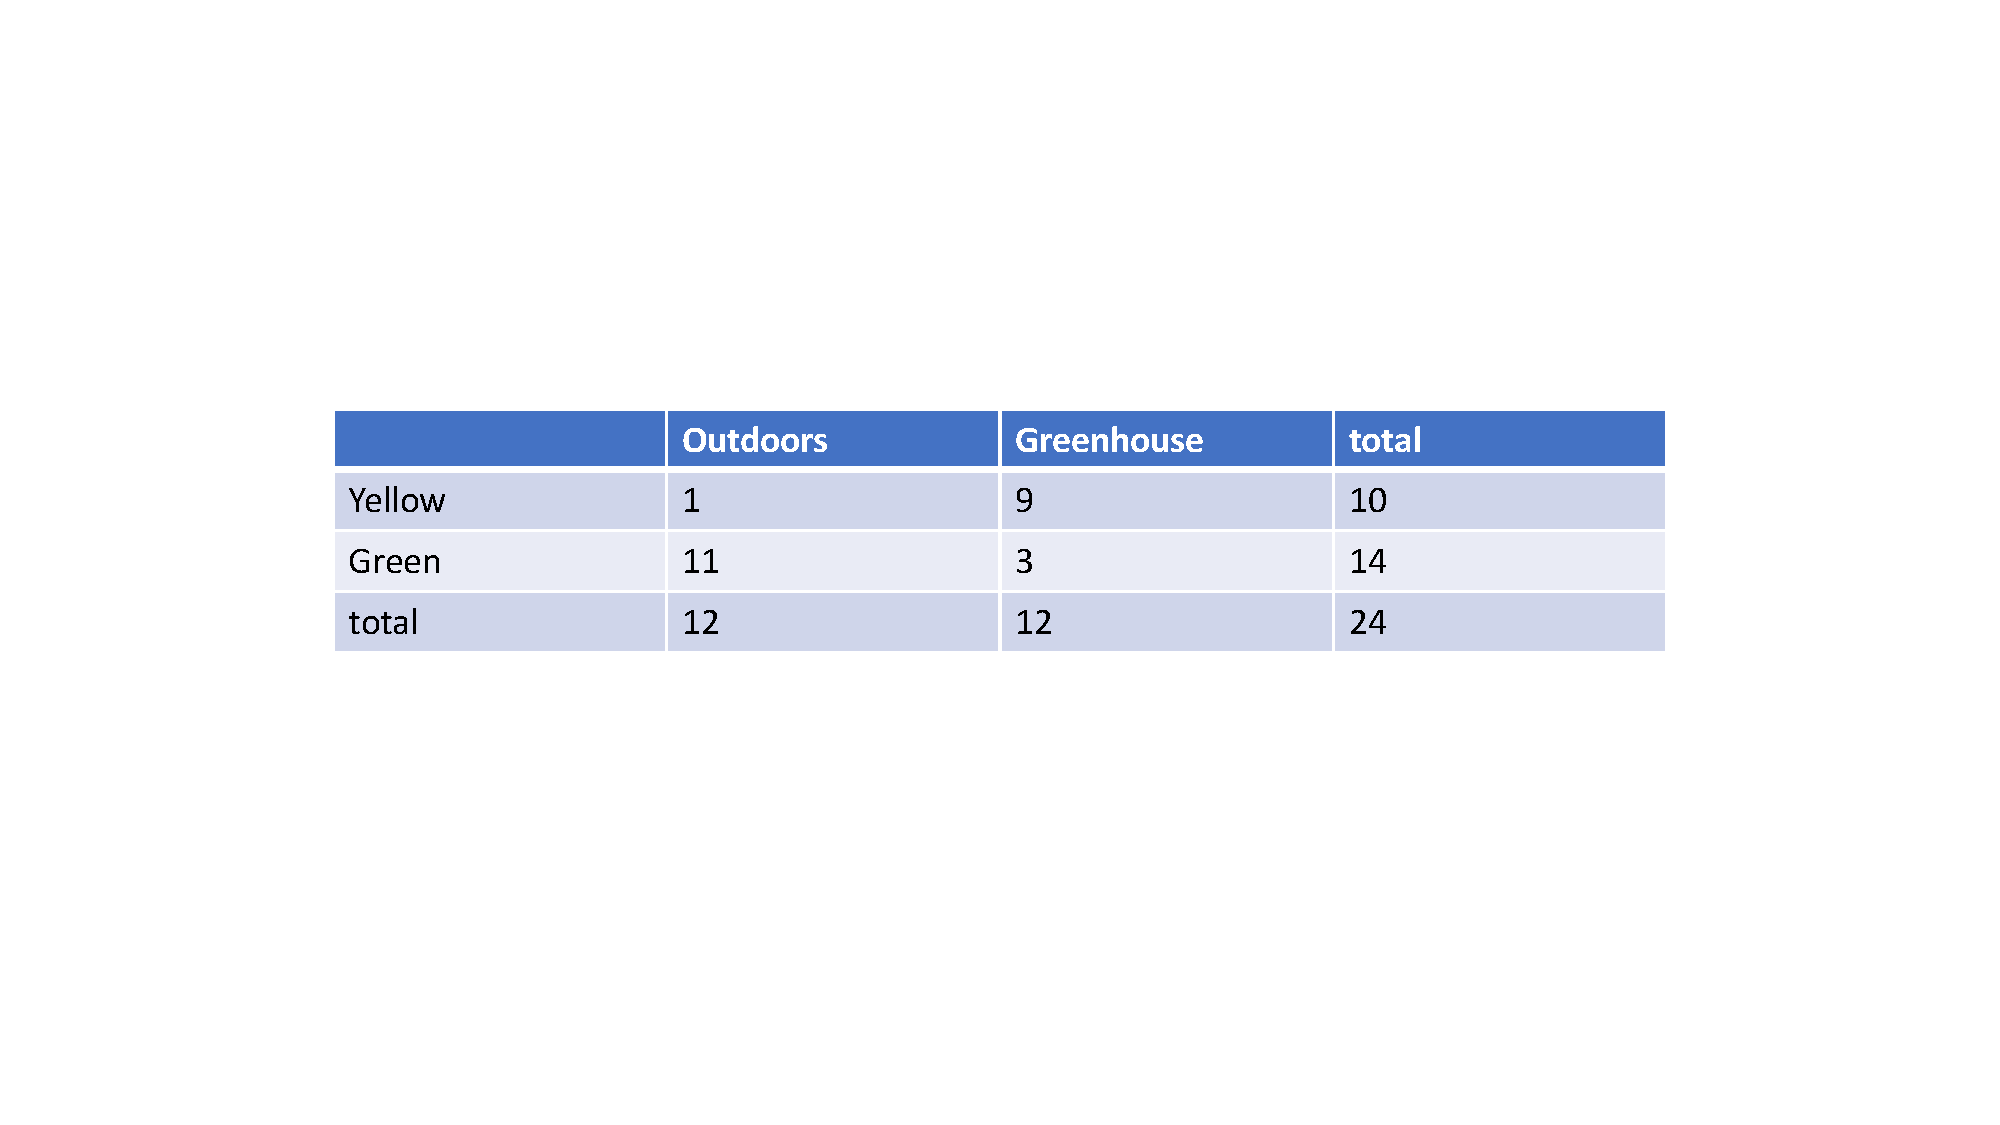
\includegraphics[width=1\textwidth]{contigencytable}

\end{frame}

\begin{frame}


\begin{block}{Example: Contingency Tables}
	
	\begin{itemize}
		\item Question: Are peas grown in the greenhouse more likely to be yellow?
		\item The test statistic in this scenarios is the hyper-geometric distribution.
	\end{itemize}
\end{block}

\begin{figure}
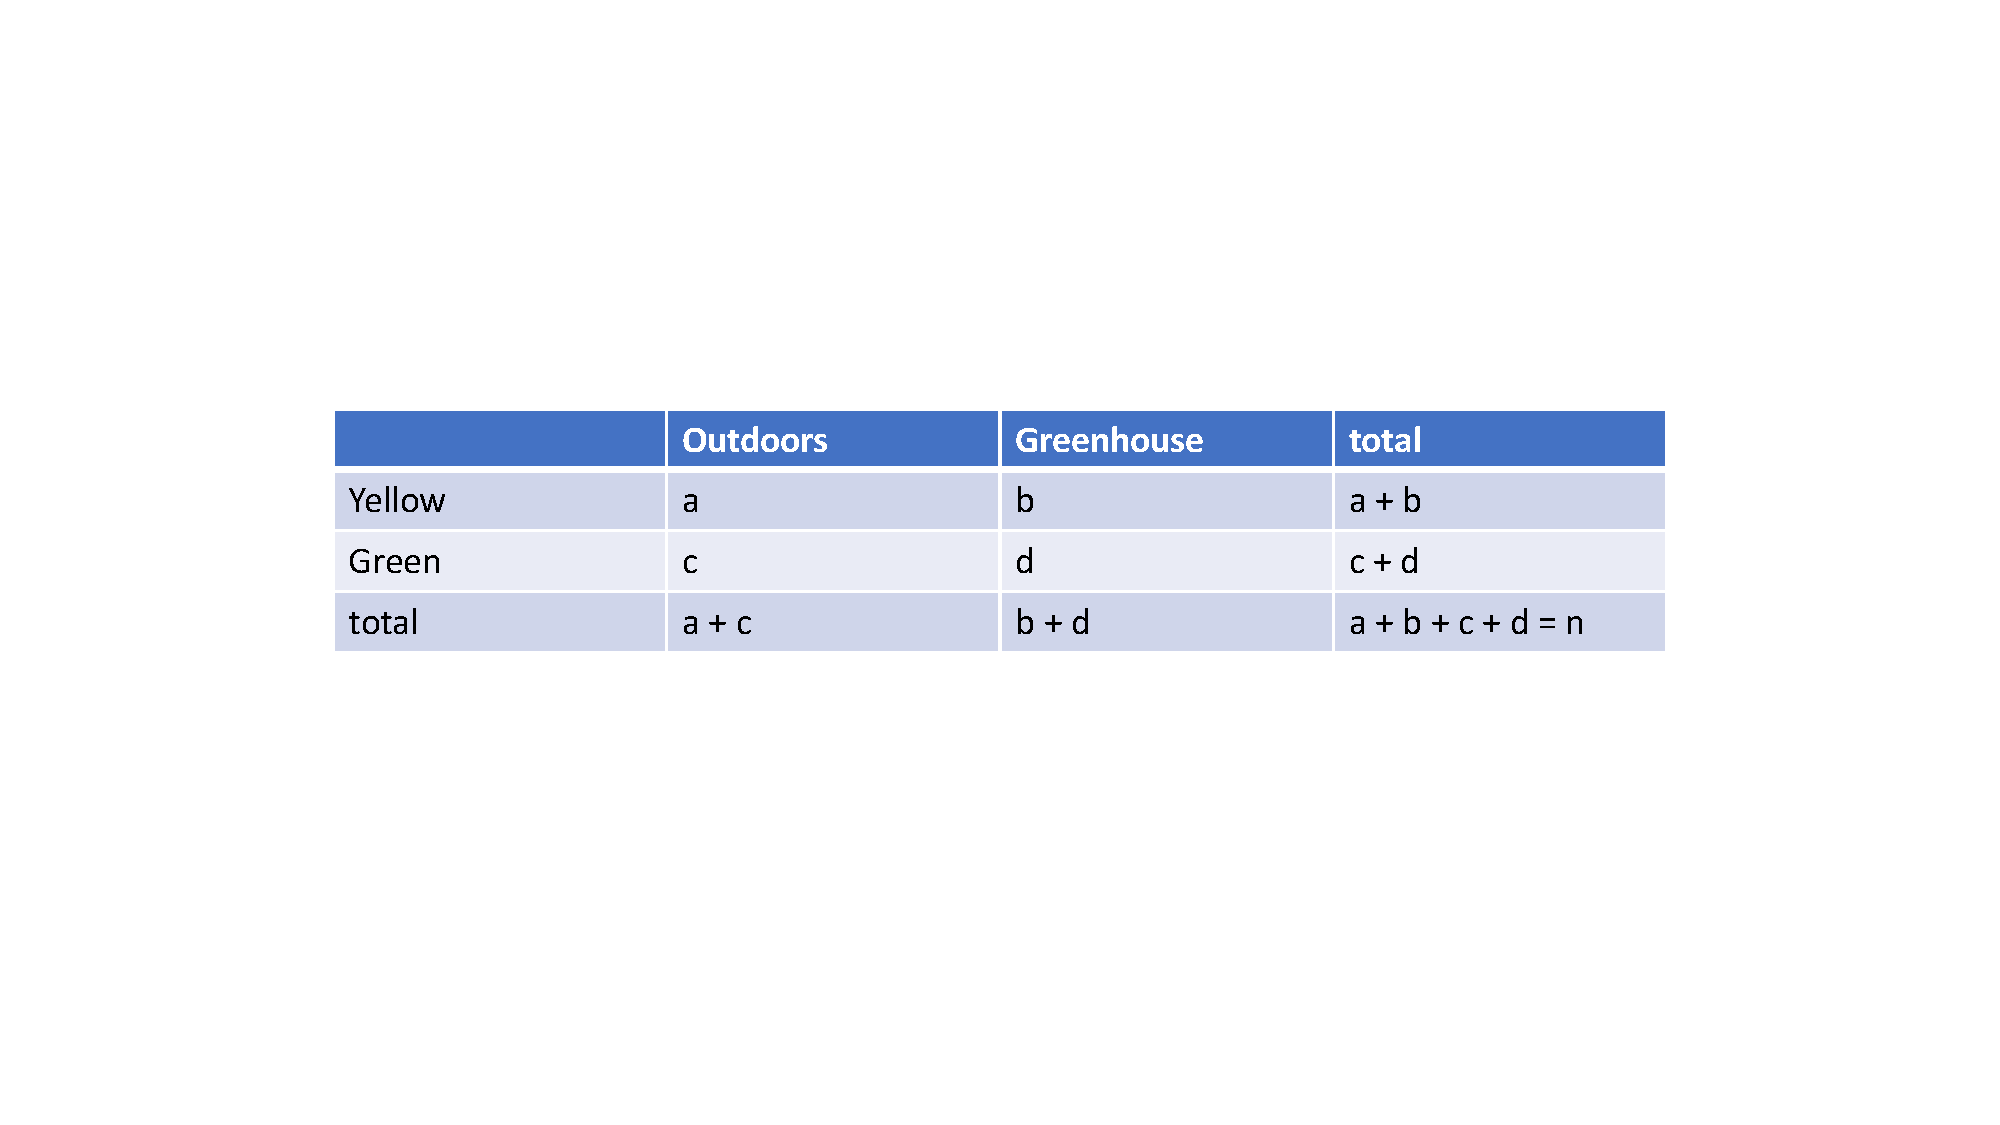
\includegraphics[width=1\textwidth]{contigencytable2}
\end{figure}

\end{frame}

\begin{frame}{The statistic}
The probability of seeing this table is
\begin{equation}
p = \frac{{a+ b \choose a} { c + d \choose c}}{{n \choose a + c}}
\end{equation}
Again, easily to use function in R. The exact refers to the fact that exact p-values are computed (no asymptotic theory).
\end{frame}

\begin{frame}{Bigger tables needs different statistics}
In this case, use the chi-squared test.

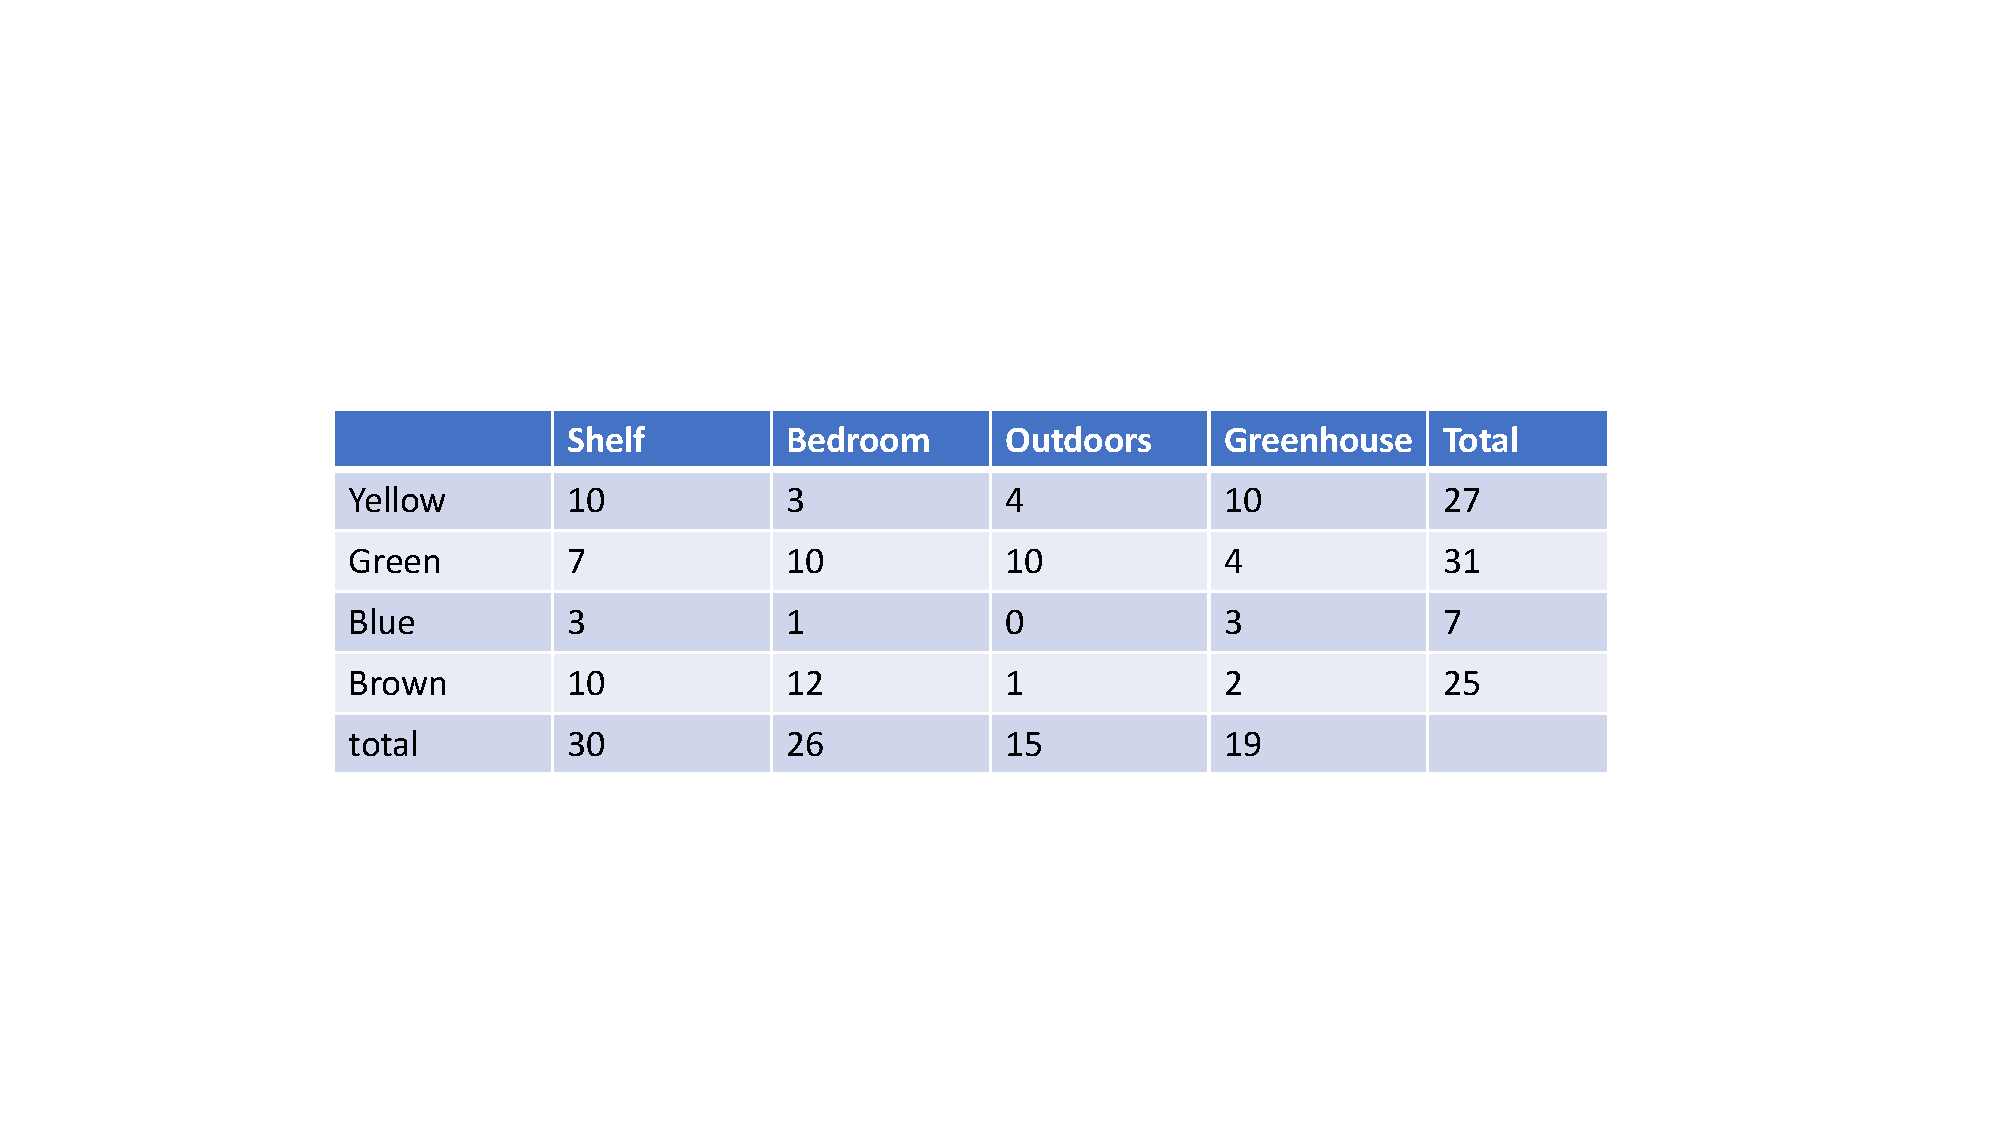
\includegraphics[width=1\textwidth]{chitable}
\end{frame}


\begin{frame}{There are many, many, many test}

\begin{block}{Many tests}
	
\begin{itemize}
\item Tukey's test
\item Wald test
\item Kolmogorov-Smirnov Test
\item Test's for normality
\item many non-parametric tests
\end{itemize}

\end{block}

\end{frame}

\begin{frame}{Permutation tests}
\begin{block}

\begin{itemize}
	
\item A general type of test that build up a sampling distribution by re-sampling from the observed data. 
\item We do this by shuffling
\item Assume we have several greenhouses with lots of plants
\item We compute the variance of the heights of plants in each greenhouse $\sigma_1^2$, $\sigma_2^2$, $\sigma_3^2$,...
\item Then we permute the plants between the greenhouses and recompute
\item Repeat this many times and we get a distribution of variance across each greenhouse
\item We can then test whether any of the greenhouse has larger variance than we would expect at random
\item Rank the $\sigma^2_1$ against the distribution of variances for greenhouse 1.
\item The p-value in this scenarios is the rank of $\sigma^2_1$ divided by the number samples
\item See example in practical

\end{itemize}
\end{block}
\end{frame}

\begin{frame}{Multiple Testing (a brief tour)}
	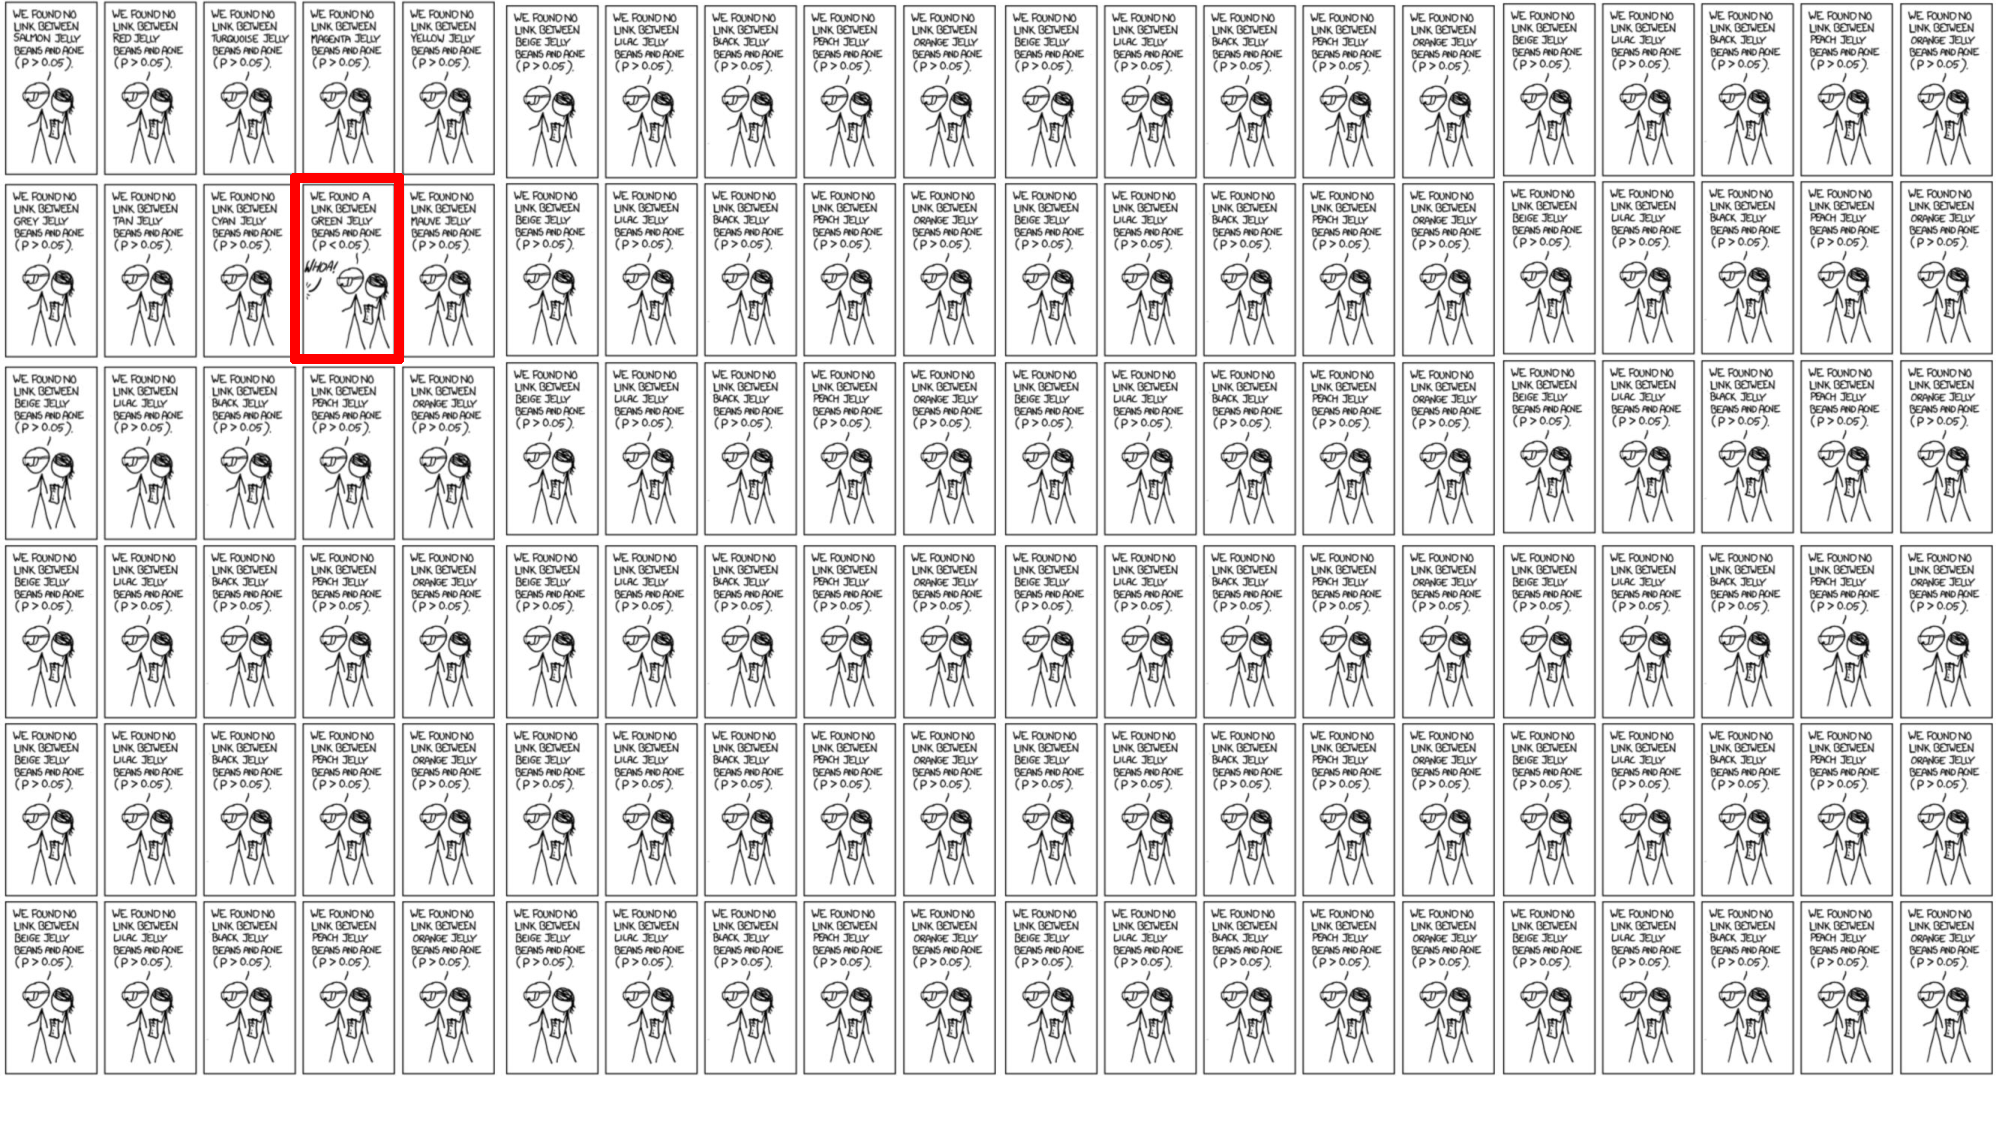
\includegraphics[width=1\textwidth]{phacking}
\end{frame}

\begin{frame}{The family wise error rate}
\begin{block}{The family wise error rate (FWER)}
Is the probability that we make one or more false positive errors.
\begin{equation}
P(V > 0 ) = 1 - P(\text{no rejection of any of } m \text{ null hypothesis}) = 1 - (1 - \alpha)^m
\end{equation}
This grows to 1 very quickly! Thus, if we are making a million test; for example, testing if two people DNA matches, then a false positive is inevitable
\end{block}
\begin{block}{Bonferroni Correction}
Bonferroni tells us that if we want to control the FWER at level $\alpha_{FWER}$, then the individual hypothesis threshold is $\alpha/m$
\end{block}
\end{frame}

\begin{frame}{The false discovery rate }
\begin{block}{p-value histogram}
\begin{itemize}
\item plot the p-value histogram
\item This is simply a histogram of the computed p-values
\item We expect a mixture distribution of two components
\item The first component corresponds to the p-values resulting from the tests for which the null hypothesis is true.
\item The second to the p-values resulting from the tests for which the null hypothesis is not true
\end{itemize}

\end{block}
\end{frame}
\begin{frame}{The p-value histogram}
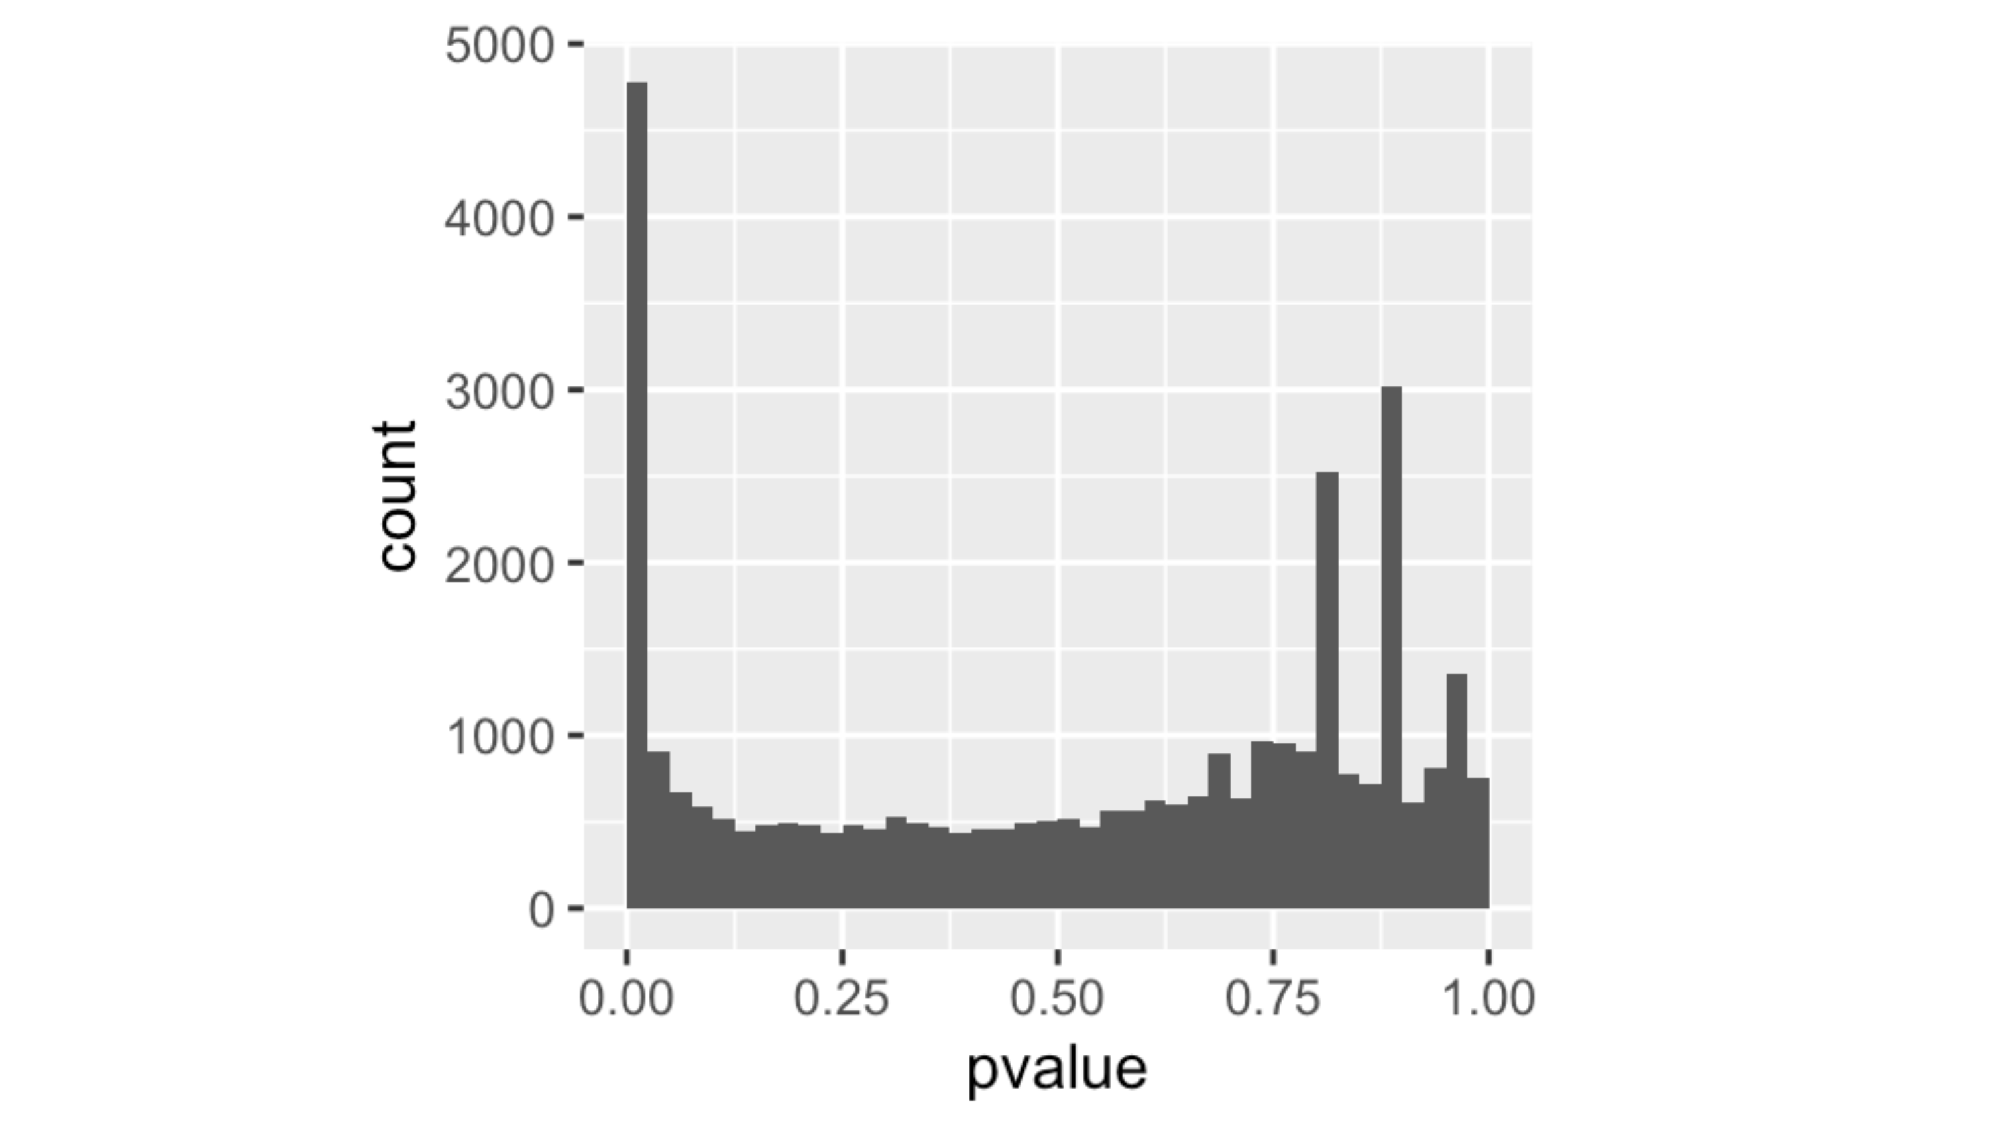
\includegraphics[width=1\textwidth]{pvaluehist}
\end{frame}
\begin{frame}{The FDR definition}
\begin{block}{False Discovery rate}
\begin{equation}
	\text{FDR } = E\left[\frac{\text{number of false positives}}{\max(\text{Number of rejections},1)} \right]
\end{equation}
\end{block}{Benjamini-Hochberg correction}
\begin{enumerate}
\item First, order the p-value in ascending order $p_1,..., p_m$
\item For a FDR theshold of level $\alpha_{FDR}$, find the largest value of $k$ such that $p_k \leq \alpha_{FDR} k /m$
\item Reject all hypothesis $p_1,...,p_k$
\end{enumerate}
\end{frame}
\begin{frame}{visualisation}
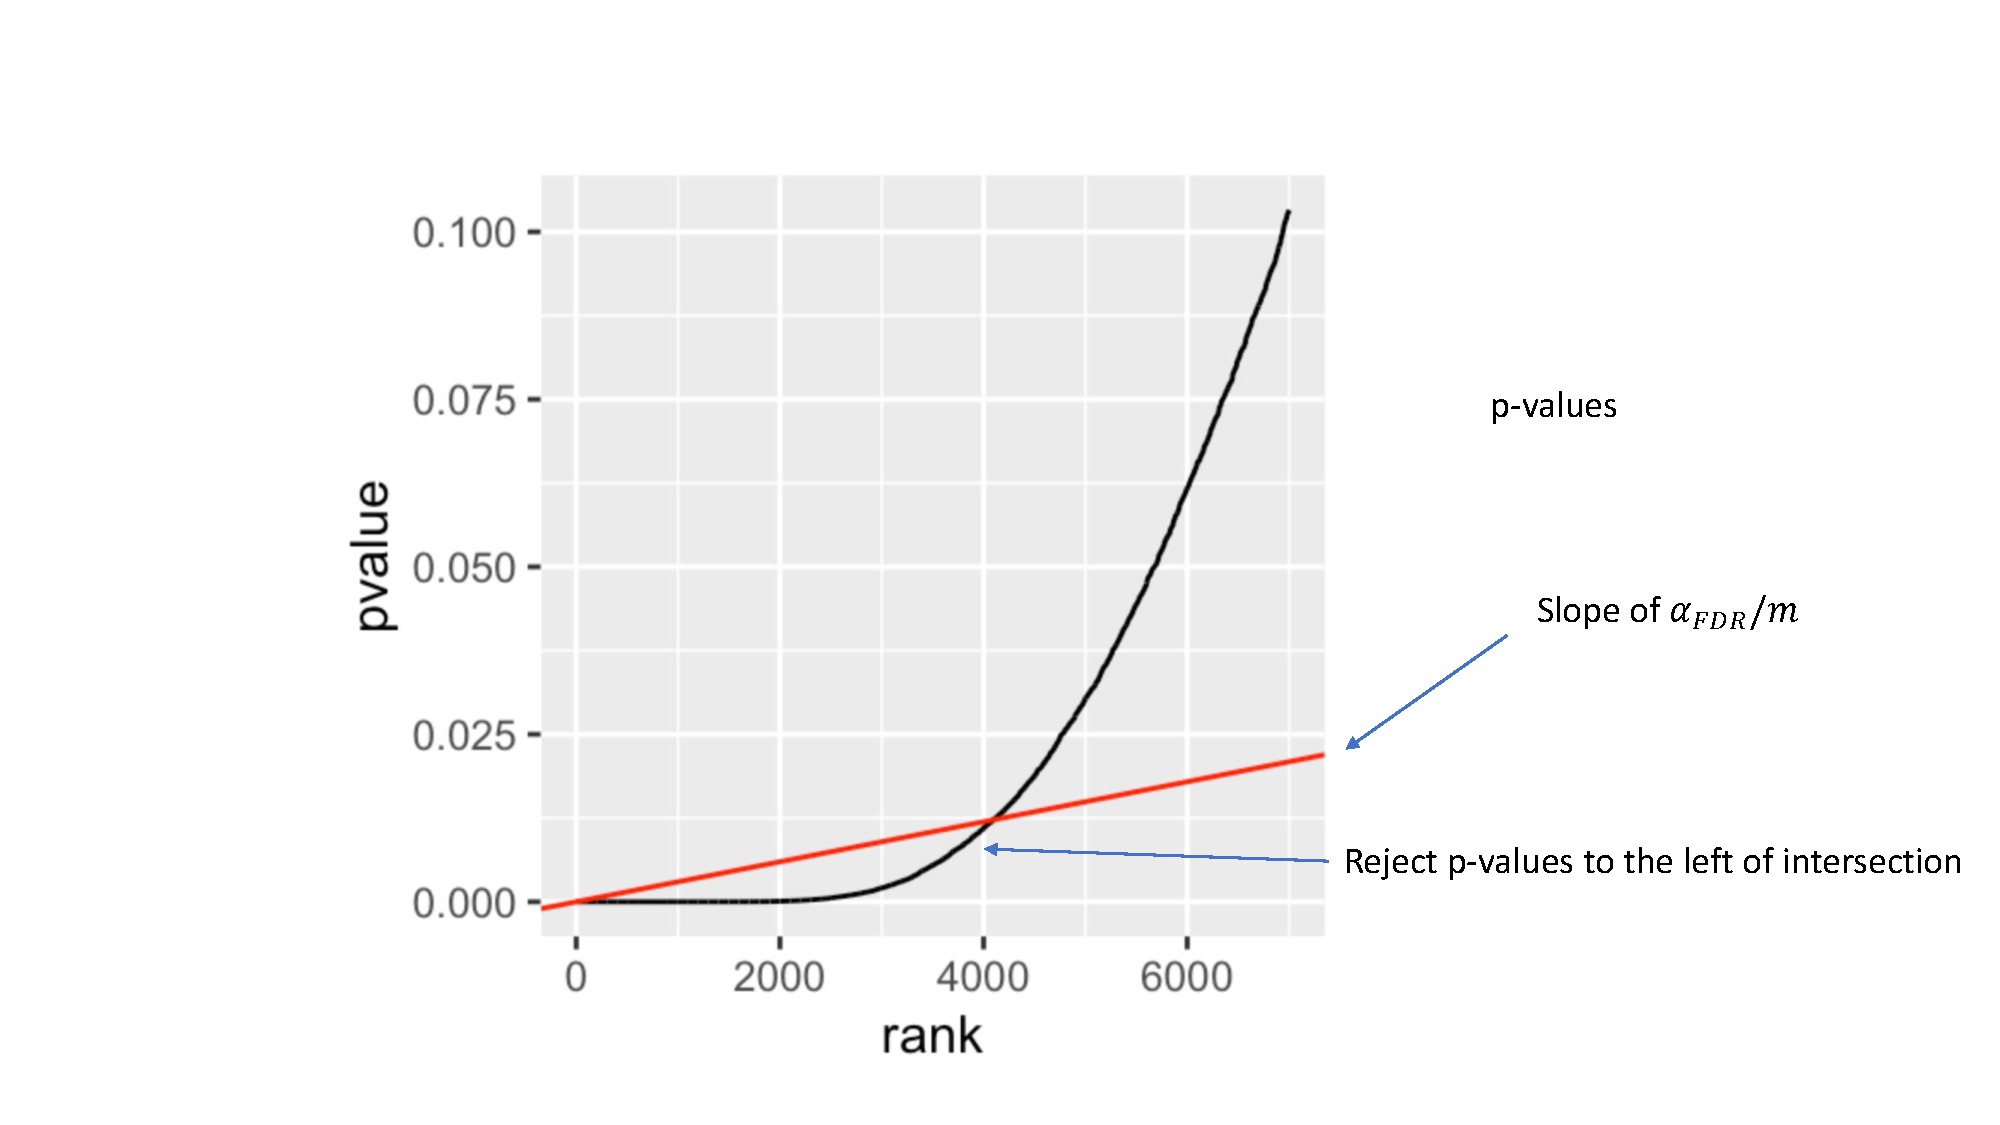
\includegraphics[width=1\textwidth]{fdrvis}
\end{frame}



\section{Linear models}
\begin{frame}{Linear models}
What is a linear regression model?
\\
A straightforward approach for predicting a quantitative response $Y$ on the basis of a variable $X$
\\
We often write
\begin{equation}
Y \approx \beta_0 + \beta_1 X
\end{equation}
\begin{block}{Observations}
\begin{itemize}
\item This is clearly a linear relationship
\item $\beta_0$ is referred to as the intercept
\item $\beta_1$ is the slope
\item Often we say that we are regressing $Y$ on $X$
\item $\beta_0, \beta_1$ are coefficients and need to be inferred from the data.
\end{itemize}
\end{block}
\end{frame}

\begin{frame}{Estimation}
\begin{block}{notation}
\begin{itemize}
	\item coefficient are unknown need to estimate them
\item estimates are given a hat e.g. $\hat{\beta}_0$
\item The predicted value of $y$ at some new points $x_*$ is given as
\begin{equation}
\hat{y} = \hat{\beta}_0 + \hat{\beta}_1x_*
\end{equation}
\item We have data $(x_1,y_1),(x_2, y_2),...,(x_n,y_n)$
\item how do we find the parameters?
\item Let $\hat{y}_i = \hat{\beta}_0 + \hat{\beta}_1x_i$ be the prediction for $Y$ based on the $i$th value of $X$.
\item Let $e_i = \text{True value } - \text{ predicted value} = y_i - \hat{y}_i$
\item we call $e_i$ the $i$th residual
\item We compute the so-called \textit{residual sum of squares} (RSS) as
\begin{equation}
RSS = e^2_1 + e^2_2 + ... e^2_n
\end{equation}

\end{itemize}

\end{block}

\end{frame}

\begin{frame}{Least squares}
The least squares method choose the coefficient $\hat{\beta}_0$ and $\hat{\beta}_1$ to minimise the RSS.
\\
This leads to
\begin{equation}
\hat{\beta}_1 = \frac{\sum_{n=1}^{n}(x_i - \bar{x})(y_i - \bar{y})}{\sum_{i=1}^{n}(x_i - \bar{x})^2}
\end{equation}
and
\begin{equation}
\hat{\beta}_0 = \bar{y} - \hat{\beta}_1 \bar{x},
\end{equation}
where the bar denotes the sample means.
\end{frame}

\begin{frame}
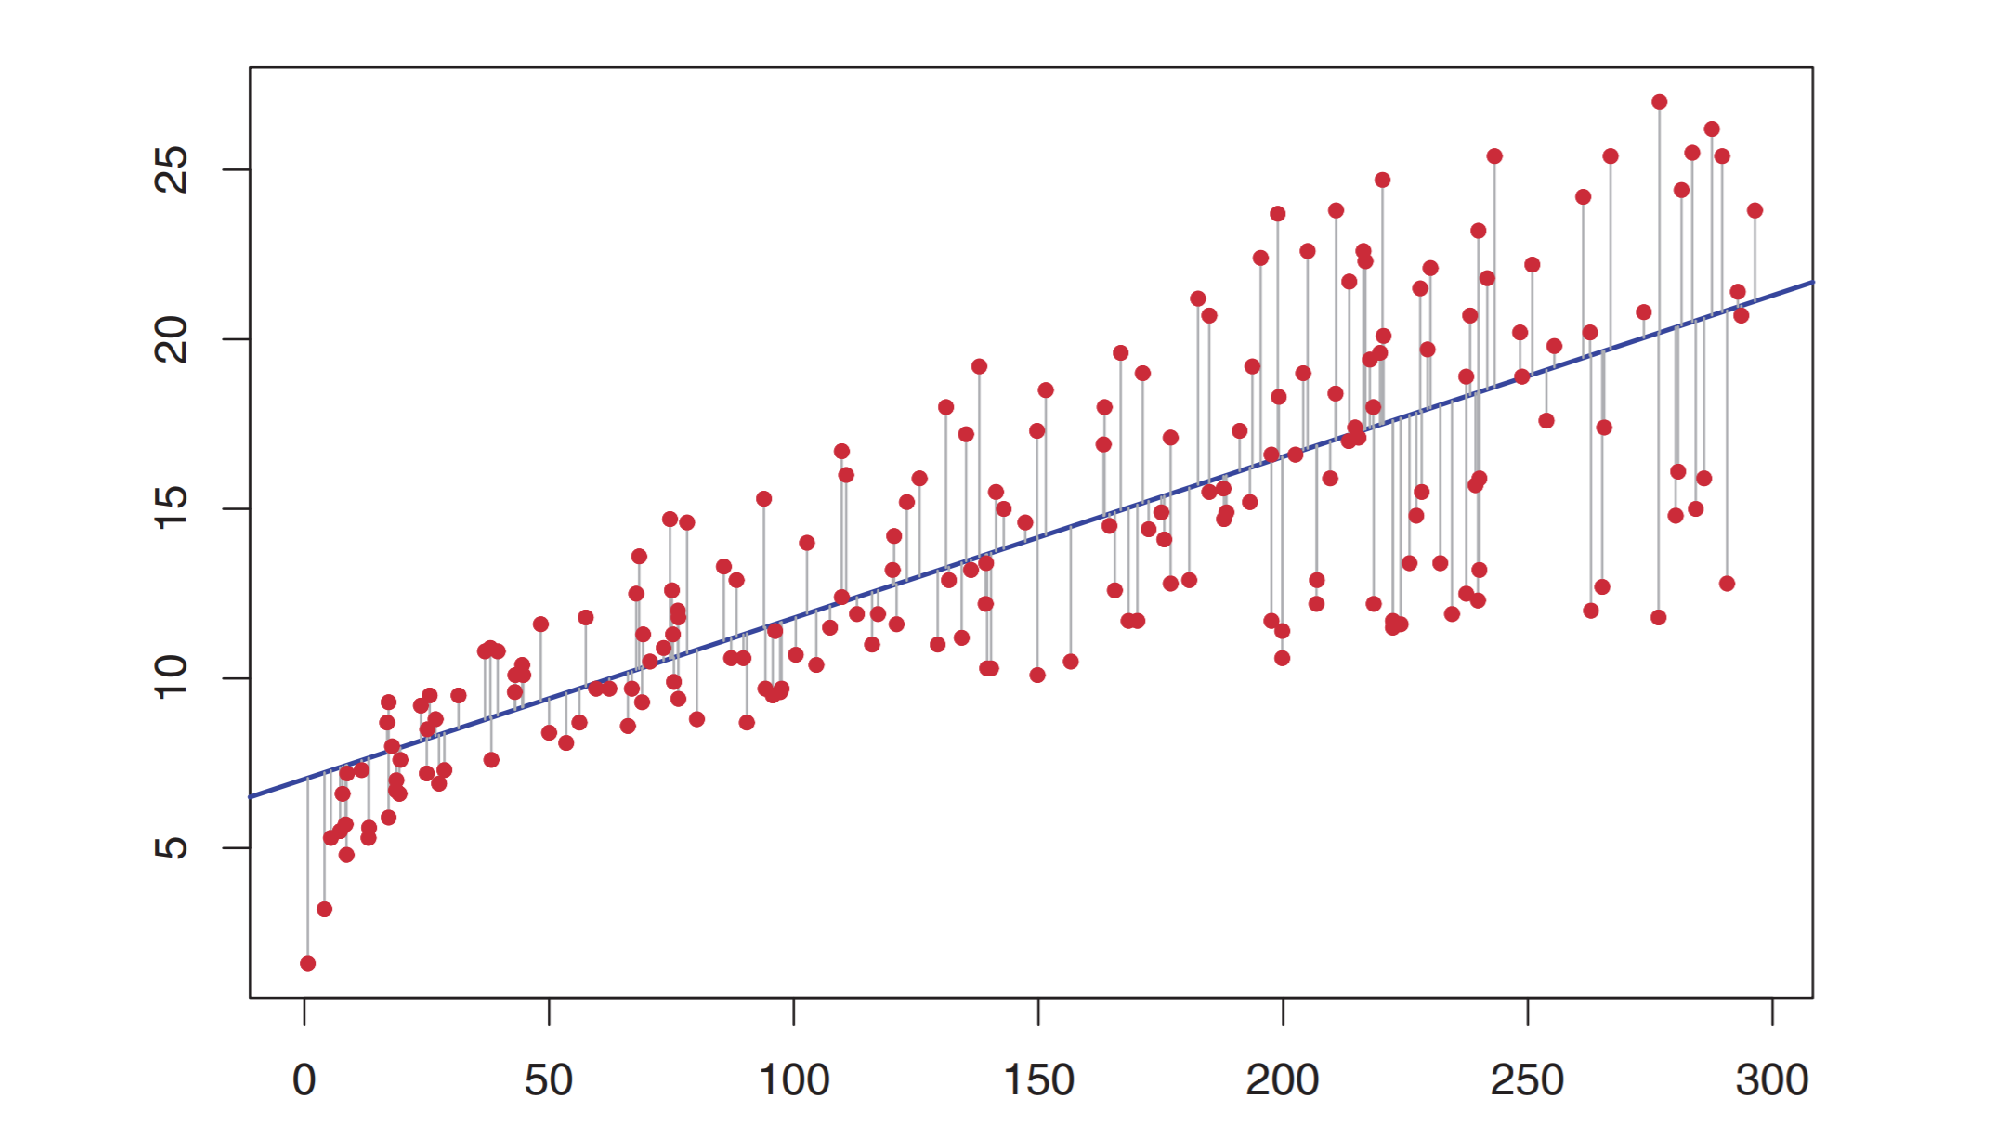
\includegraphics[width=1\textwidth]{linearregression}
\end{frame}
\begin{frame}{How good is by approximation?}
A more formal problem set-up is that our observation arise from a linear model but are then corrupted by independent noise
\begin{equation}
Y = \beta_0 + \beta_1X + \epsilon,
\end{equation}
where 
\begin{equation}
\epsilon \sim \mathcal{N}(0, \sigma^2)
\end{equation}
(the tilde/squiggle means distributed as)
\\
We can now ask how close are $\hat{\beta}_0$ and $\hat{\beta}_1$ to the "true" $\beta_0$ and $\beta_1$?
\\
We can compute the standard errors (SE):
\begin{equation}
SE(\hat{\beta}_0)^2 = \sigma^2\left[\frac{1}{n} + \frac{\bar{x}^2}{\sum_{i = 1}^{n}(x_i - \bar{x})^2} \right]
\end{equation}
and
\begin{equation}
SE(\hat{\beta}_1)^2 =  \frac{\sigma_1^2}{\sum_{i =1 }^{n}(x_i - \bar{x})^2}
\end{equation}

\end{frame}

\begin{frame}{Confidence Intervals}
For linear regression, we can now compute the $95\%$ confidence interval
\begin{equation}
\hat{\beta}_1 \pm 2 SE(\hat{\beta}_1)
\end{equation}
We say that the the true value of $\beta_1$ has a $95 \%$ chance of falling into the interval.
\begin{equation}
\left[\hat{\beta}_1 - 2 SE(\hat{\beta}_1), \hat{\beta}_1 + 2 SE(\hat{\beta}_1)\right]
\end{equation}

\begin{alertblock}{warning}
	The $2$ in front of the standard error means that this is only approximate. We actually need to put the $97.5\%$ quantile of a t-distribution with $n-2$ degrees of freedom (more later)
\end{alertblock}

\end{frame}

\begin{frame}{linear models as a Hypothesis test}
We might want to test the following hypothesis
\begin{equation}
H_0: \text{There is no relationship between } X \text{ and} Y 
\end{equation}
and
\begin{equation}
H_a: \text{There is some relationship between } X \text{ and} Y 
\end{equation}
This is equivalent to 
\begin{equation}
H_0: \beta_1 = 0
\end{equation}
and
\begin{equation}
H_1: \beta_1 \neq 0
\end{equation}
\end{frame}

\begin{frame}
As we've seen before we need to see whether our estimate $\hat{\beta}_1$ is sufficiently far from $0$. We compute the statistic
\begin{equation}
t = \frac{\hat{\beta}_1 - 0 }{SE(\hat{\beta}_1)}
\end{equation}
(This is our good old friend the t-statistics).
\\
\begin{block}
	
\begin{itemize}
\item If there really is no relationship between $X$ and $Y$, then the above statistics has a t-distribution with $n - 2$ degrees of freedom.
\item You can then calculate the p-value (using pt in R).
\item Intuitively we are concerned about whether the magnitude of the coefficients are much bigger than the standard error.
\end{itemize}
\end{block}
\end{frame}

\begin{frame}{Goodness of fit}
How good is our model of the data?
\begin{exampleblock}{$R^2$}
	\begin{itemize}
		\item Many ways to measure model fit 
		\item How much variance does our model explain?
		\item Want quantity to be independent of the scale of the data
		\item $R^2$ measures the proportion of variance explained by a model
		\begin{equation}
		R^2 = \frac{\text{TSS } - \text{RSS}}{\text{TSS}}
		\end{equation}
		where
		\begin{equation}
		\text{TSS} = \sum_{i = 1}^{n} (y_i - \bar{y})^2
		\end{equation}
		\item $R^2$ measure the proportion of variability in $Y$ that can be explained using $X$
		\end{itemize}
\end{exampleblock}
\end{frame}

\begin{frame}{Multiple Regression}
We have only worked with one predictor but in reality we have more than 1 predictor. For example, the height of plant is a function of both amount of sun and amount of water (and whether or not nutrients were added etc)
\begin{exampleblock}{multiple regression}
\begin{itemize}
\item Suppose we have $p$ possible predictors (variables that may effect our outcome)
\begin{equation}
Y = \beta_0 + \beta_1X_1 + \beta_2X_2 + ... + \beta_p X_p + \epsilon
\end{equation}
\item The least squares approach (i.e. minimising the RSS) can be used to estimate parameters
\end{itemize}
\end{exampleblock}
\end{frame}

\begin{frame}{Multiple Regression questions}

\begin{exampleblock}{multiple regression questions}
	
	\begin{itemize}
\item Is at least one predictor useful for predicting the response?
\item Are a subset of predictors useful?
\item Model fit?
	\end{itemize}
\end{exampleblock}
\begin{block}{Answers}
	
	\begin{itemize}
		\item This is part of variable selection and can use criterion such as BIC and AIC
		\item More sophisticated variable selection methods (time restriction)
		\item The $R^2$ can be used to assess model fit as before
	\end{itemize}

\end{block}
\end{frame}


\begin{frame}{Hypothesis for multiple regression}
\begin{block}{Are of of my predictors useful?}
	
\begin{equation}
H_0: \beta_1 = \beta_2 = \beta_3 = ... = \beta_p = 0
\end{equation}
against
\begin{equation}
H_a: \text{ at least one of $\beta_j$ is non-zero}
\end{equation}
We need a more complicated test statistics. We compute
\begin{equation}
F = \frac{(\text{TSS - RSS})/p}{RSS/(n - p - 1)}
\end{equation}
large values of $F$ indicate evidence against the null. But what about p-values?
unsurprisingly, the F-statistic follows the F-distribution (pf in R)
\end{block}
\begin{alertblock}{warning}
 Why didn't wee test each variable separately using the t-statistic?
\end{alertblock}
\end{frame}

\begin{frame}{Linear models with factors}
Up until this point we have only considered linear models with quantitative variables. We can also include factors, such as treated or untreated, male or female, Human or mouse etc.
\begin{exampleblock}{factors}

Consider plant height with treatment or no treatment of fungicide 
\\
 $x_i = 1$ if treated $x_i = 0$ not treated
\begin{equation}
y_i = \beta_0 + \beta_1x_i + \epsilon_i
\end{equation}
 $\beta_0$ is now interpreted as treated average height of untreated plants
 \\
 $\beta_0 + \beta_1$ is the average height of treated plants
 \\
 $\beta_1$ is the average difference in heights between the treated and untreated

\end{exampleblock}

\begin{alertblock}{Question}
How do I test if the treatment has an effect on height?
\end{alertblock}

\end{frame}

\begin{frame}{Linear models with more factors}
Suppose there are now two possible treatments.
\begin{exampleblock}{Multiple factors}
	Use the $0$ or $1$ coding for each treatment
	\begin{equation}
	y_i = \beta_0 + \beta_1x_{i1} + \beta_2x_{i2} + \epsilon_i
\end{equation}
How do I interpret these coefficients?
\\
Does a treatment improve height? Use the F-statistic for 
\begin{equation}
H_0: \beta_1 = \beta_2 = 0 
\end{equation}
\end{exampleblock}
\end{frame}
\begin{frame}{Interaction effects}
What if we think that the two treatments together my have an additional \textit{iteraction} effect
\begin{exampleblock}{Multiple factors and interaction effects}
	Use the $0$ or $1$ coding for each treatment, include an additional product term.
	\begin{equation}
	y_i = \beta_0 + \beta_1x_{i1} + \beta_2x_{i2} + \boldsymbol{\beta_3x_{i1}x_{i2}} + \epsilon_i
	\end{equation}
	The coefficient $\beta_3$ explains the additional effect of having both treatments over the additive benefit of each individual treatment
	\\
	We can apply all the machinery we've done before. For example we can test to see whether $\beta_3$ is significant and conclude there is an interaction effect.
\end{exampleblock}
\begin{alertblock}{Warning: The hierarchical principle}
	If we include an interaction in a model, we also include the main effects, even if the p-values associated with their coefficients are not significant.
\end{alertblock}

\end{frame}

\begin{frame}{Further Models}
To cover sufficient breadth, we missed out some important topics.
\begin{exampleblock}{linear models are linear in the parameters}
	The following is a linear model, even though there is a non-linear transformation of the predictors
\begin{equation}
	y_i = \beta_0 + \beta_1x_{i1}^2 + \beta_2 \sin(x_{i
2}) + \beta_3 x_{i1}\sin(x_{i2}) + \epsilon_i
\end{equation}
\end{exampleblock}
\begin{exampleblock}{The response may more complex}
	The following is an example of binomial regression, where the outcome responses
	are binomially distributed
	\begin{equation}
	y_i = \text{Binom}\left(n_i, \frac{1}{1 + \exp(- \beta_1x_{i1} - \beta_2x_{i2})}\right)
	\end{equation}
	Further, complex models can be included in this framework known a \textit{generalised linear models}
\end{exampleblock}

\end{frame}

\section{Dimensionality Reduction}

\begin{frame}{Dimensionality Reduction}
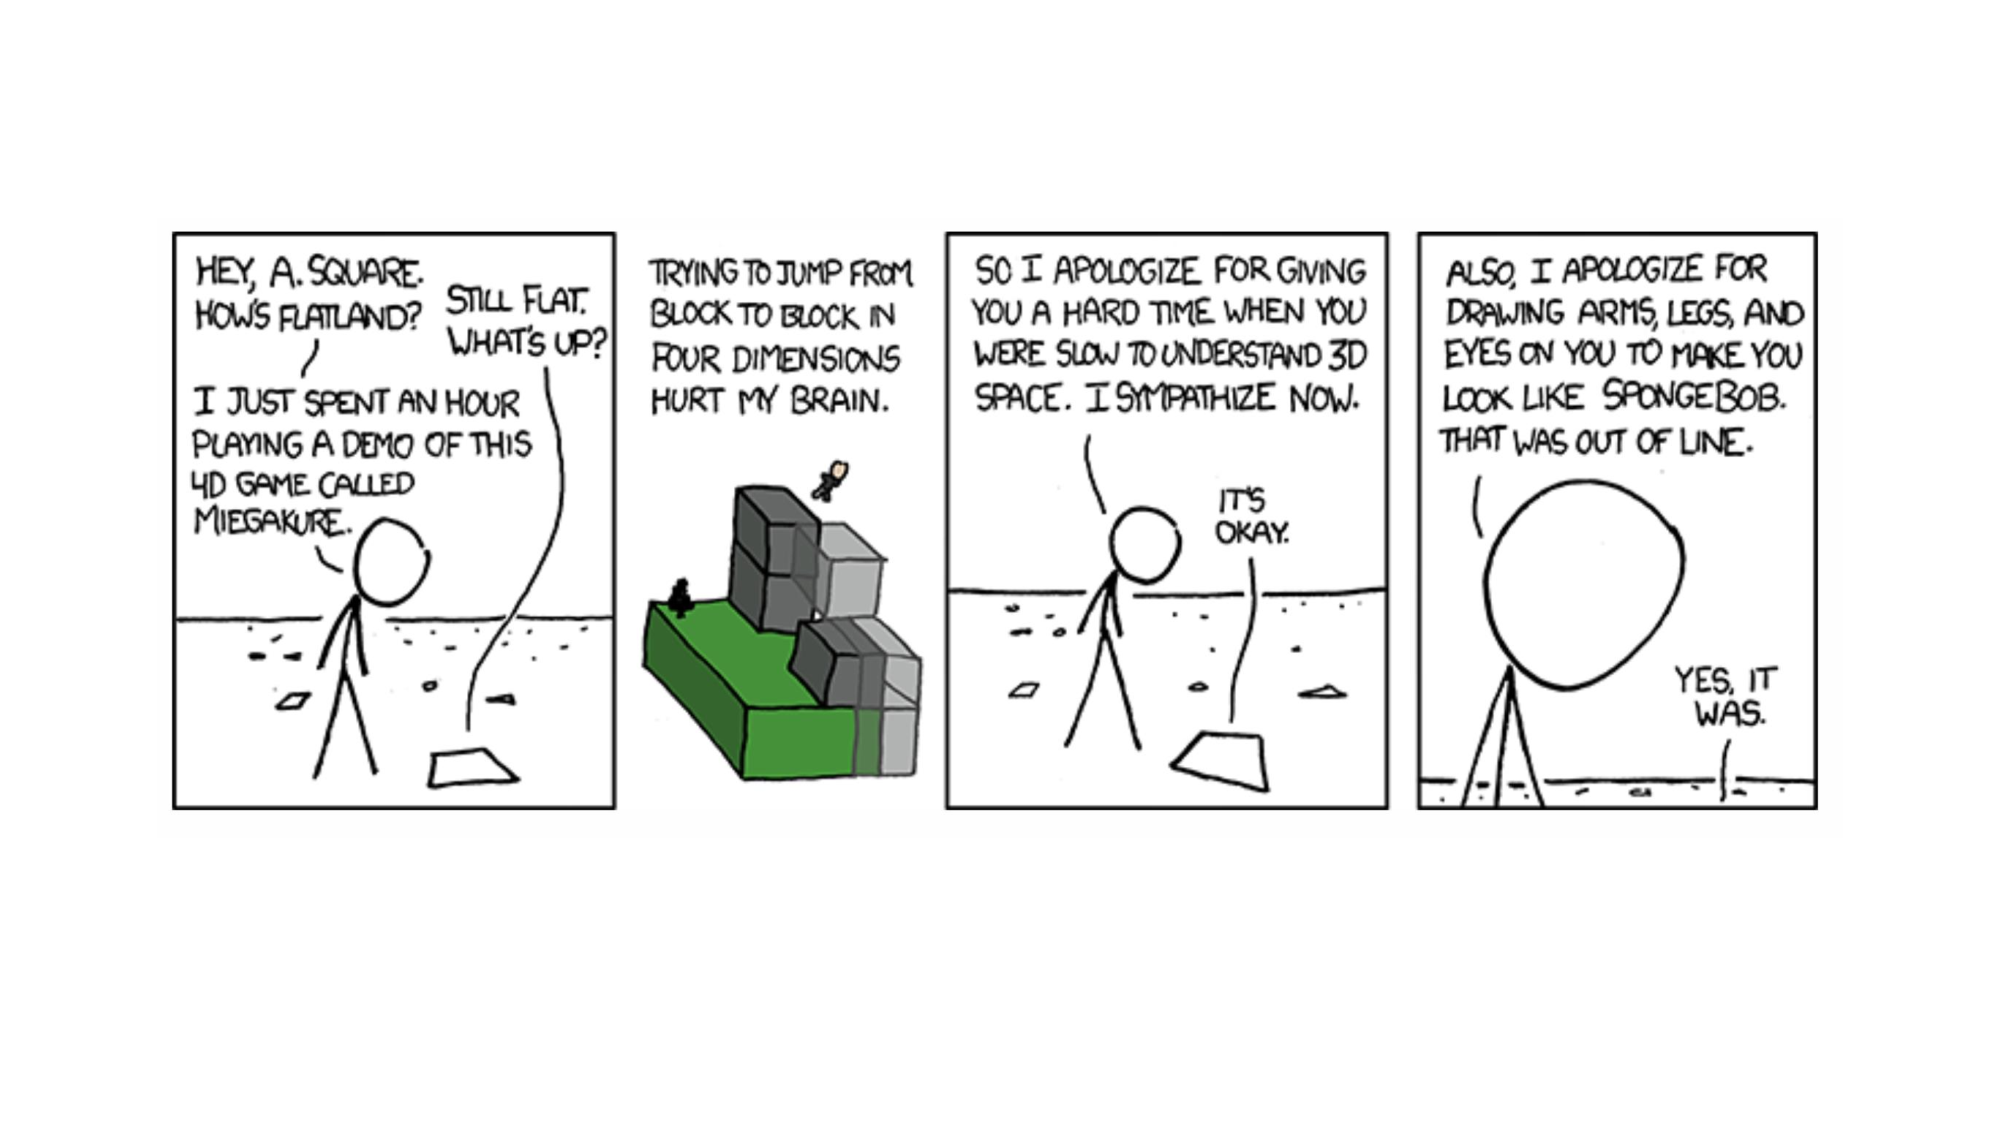
\includegraphics[width=1\textwidth]{dimreduce}
\end{frame}

\begin{frame}{Dimensionality Reduction}
\begin{block}{Aims}
\begin{itemize}
\item Visualise high-dimensional data
\item Reduce high-dimensional data into a more manageable size
\item Understanding the variation in the data.
\end{itemize}
\end{block}

\begin{alertblock}{Warnings}
\begin{itemize}
\item Are we applying the correct dimensionality reduction tool?
\item Yes, it looks nice ... but is it useful?
\item Visualisations should tell you something about the data, not what you'd like to data to show you 
\end{itemize}
\end{alertblock}

\end{frame}

\begin{frame}{Principal Component Analysis}
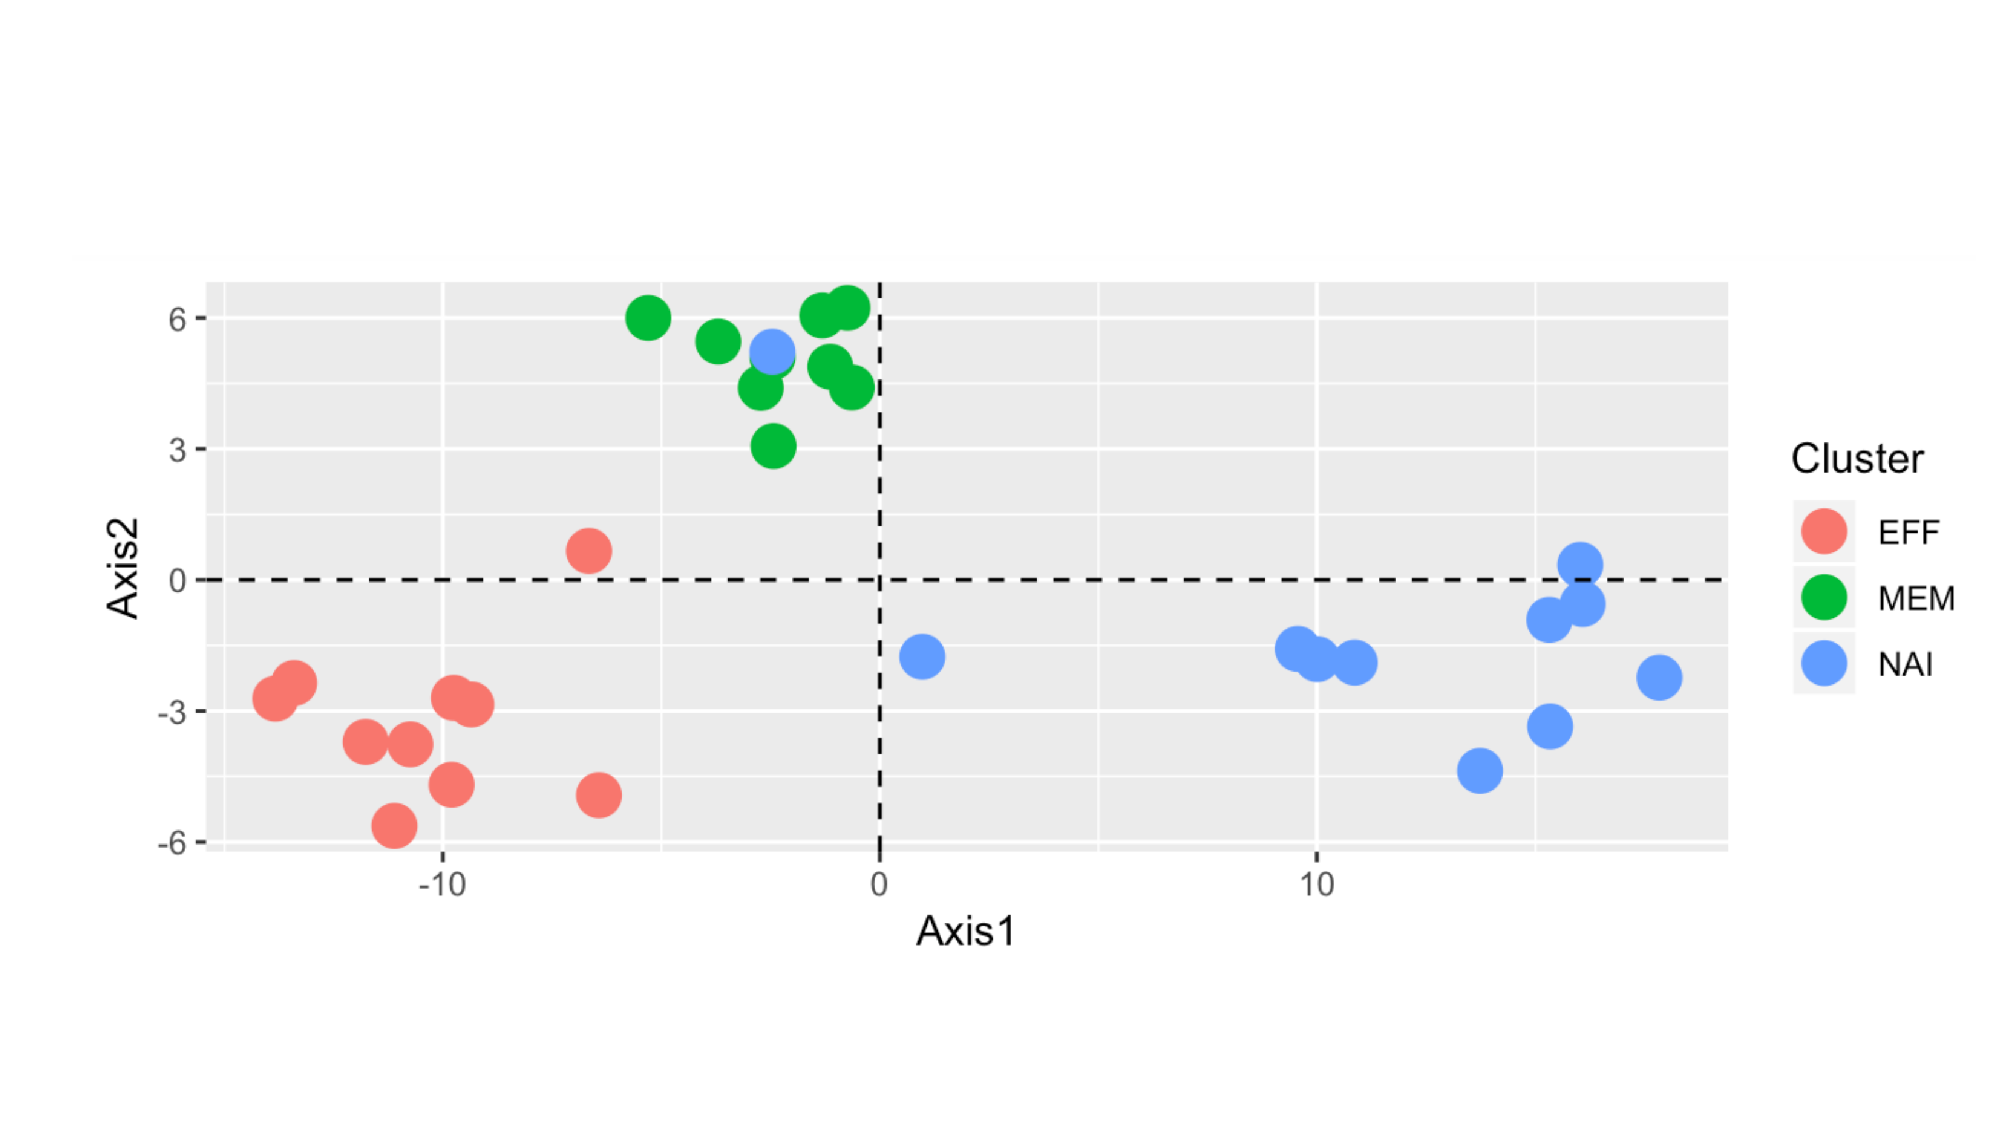
\includegraphics[width=1\textwidth]{pcaplot}
\end{frame}

\begin{frame}{Principal Component Analysis}
\begin{exampleblock}{PCA}
\begin{itemize}
\item Unlike regression PCA only involves features $X_1,X_2,...,X_p$(and no response)
\item PCA can be used to visualise observation or variables.
\item Is applicable to continuous data.
\item We would like to project the data in direction of greatest variability
\item Look at linear combinations, which maximise sample variance
\begin{equation}
z_{i1} = \phi_{11}x_{i1} + \phi_{21}x_{i2} + ... + \phi_{p1} x_{ip}
\end{equation}
\item $z_{11},...,z_{n1}$ are known as \textit{scores} (of the first principal component)
\item $\phi_1,..., \phi_p$ are referred to as \textit{loadings}
\item Subsequent principal components look for maximal variance but are also orthogonal(uncorrelated) to previous principal components
\end{itemize}
\end{exampleblock}
\end{frame}
\begin{frame}{Principal Component Analysis}
\begin{exampleblock}{Variance and variables}
	\begin{itemize}
	\item We can compute how much variance is explained by each principal component
	\begin{itemize}
	\item Compute the overall variance of the data (for each feature)
	\begin{equation}
	var(X_1),..., var(X_p)
	\end{equation}
	\item Compute the the variance of the scores for each component
	\begin{equation}
	var(z_1),..., var(z_m)
	\end{equation}
	\item The proportion of variance explain by the th $j$th component is the variance of that component divided by the total variance.
	\begin{equation}
	VE_j = \frac{var(z_j)}{\sum_{i =1}^{p} var(X_i)}
	\end{equation}
	\end{itemize}
	\end{itemize}
\end{exampleblock}

\begin{alertblock}{batch Effects}
If a large proportion of variance is explained by an experimental day, machine type etc - you have a batch effect. (More later). These can often be found using PCA.
\end{alertblock}

\end{frame}


\begin{frame}{Correspondence Analysis}

\begin{exampleblock}{Aims}
	
	\begin{itemize}
\item Dimensionality reduction applied to contingency tables
\item Uses the chi-squared distance
\item As with PCA can be used to explain variability.
\item I won't go into the mathematics here
\item Many other dimensionality reduction tools
\end{itemize}
\end{exampleblock}
\end{frame}

\begin{frame}{Correspondence Analysis}

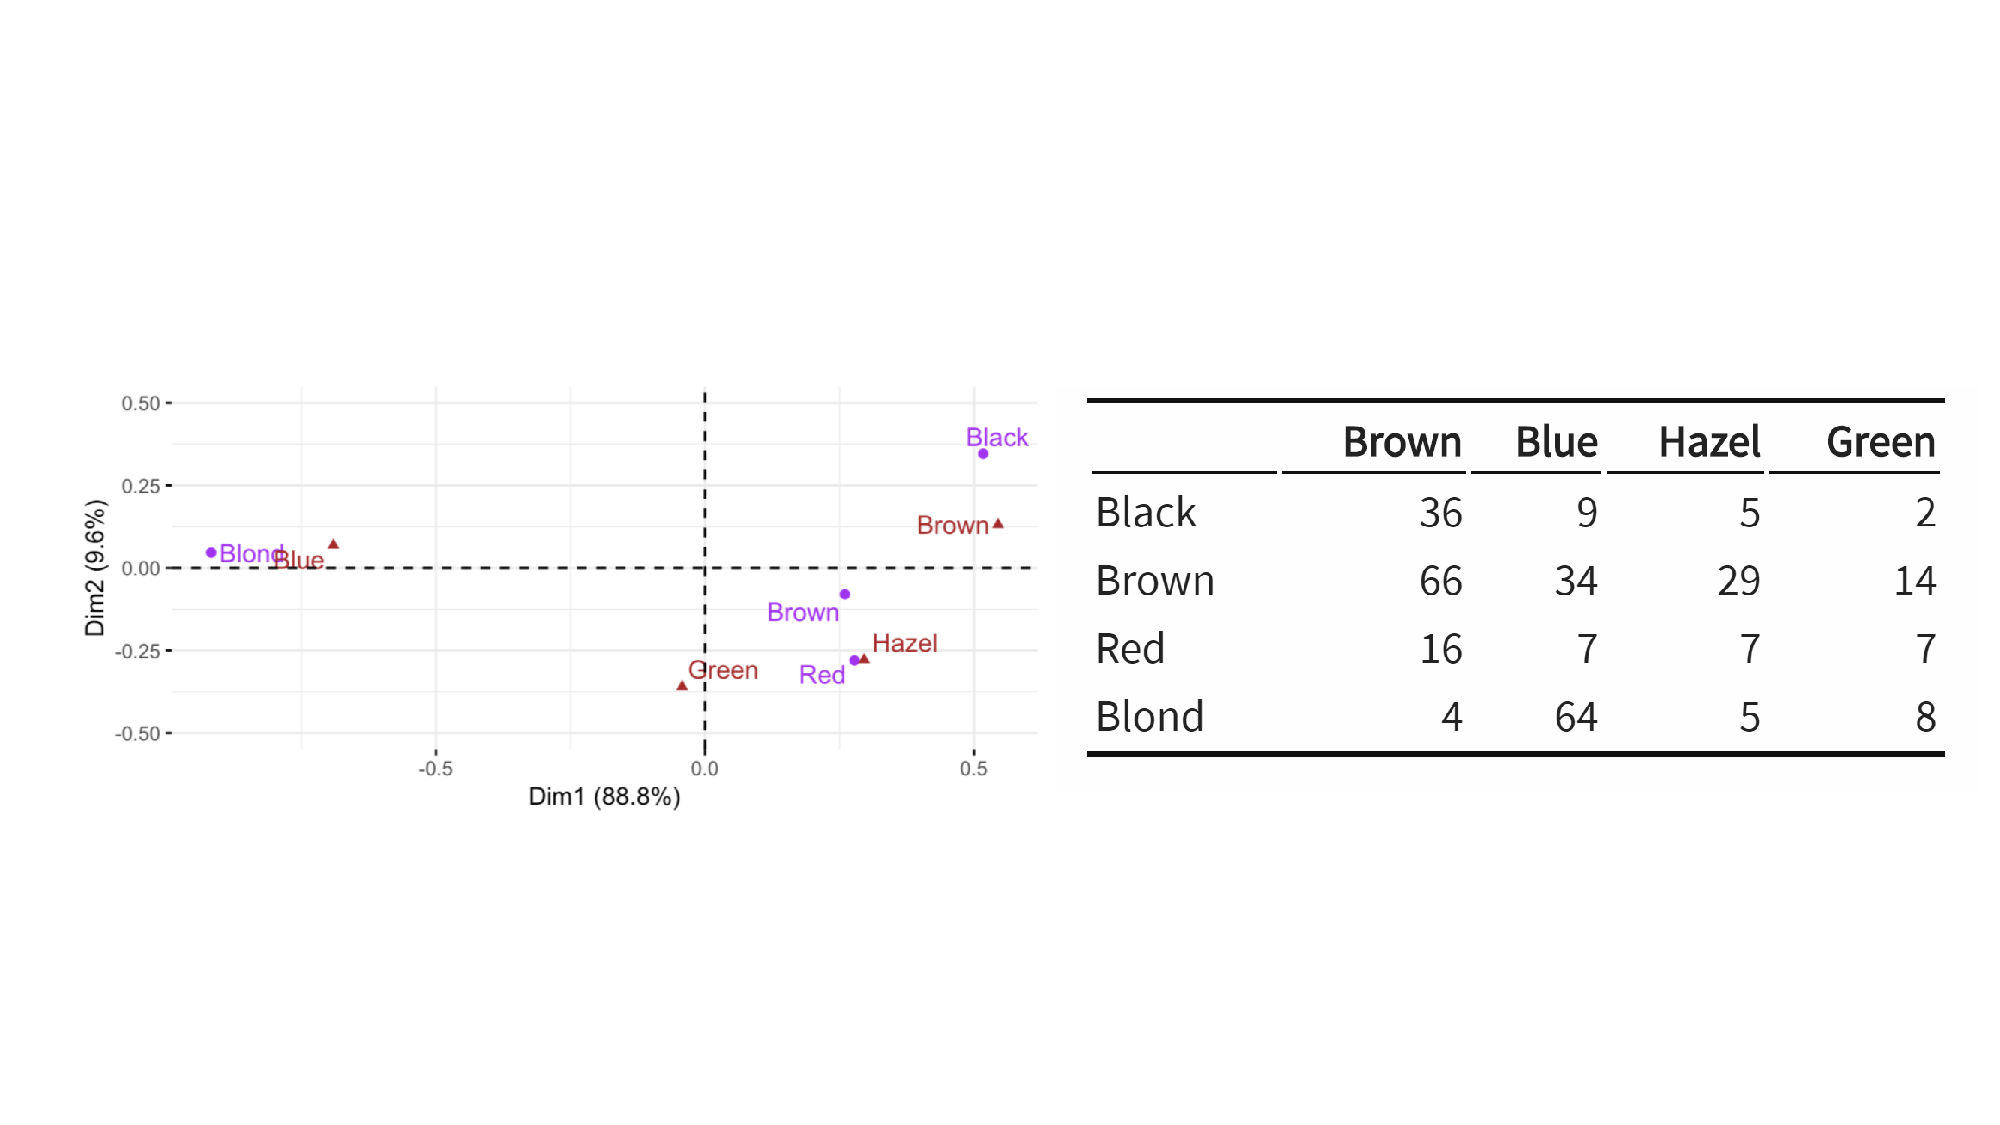
\includegraphics[width = 1\textwidth]{corranalysis}
\end{frame}

\section{Classification}


\begin{frame}{Classification}

\begin{exampleblock}{Goals}
	
\begin{itemize}
	
\item Many statistical and machine learning tasks require the prediction of labels from data (and some already labelled data)
\item This might be cell type, country of origin, sex, broken or not etc.
\item There are MANY methods, logistics regression, K-NN, SVM, Deep learning etc
\end{itemize}

\end{exampleblock}

\end{frame}


\begin{frame}{K-nearest neighbours}

One of the simplest classification algorithms, is the k-nearest neighbours (KNN). It is a non-parametric approach.
\begin{exampleblock}{KNN}
	
	\begin{itemize}
		
		\item Suppose our data $X$ can take label $y_i = 1,..., J$
		\item Imagine a portion of these data already have labels
		\item Suppose we have a point $x_i$ without a label
		\item Assign a label by looking at the $K$ closest points with labels
		\item Probabilistically we can think of assigning the label with maximal probability
		\begin{equation}
		Pr(y_i = j|X = x_i) = \frac{1}{K}\sum_{l \in \mathcal{N}_i}I(y_l = j),
		\end{equation}
		where $\mathcal{N}_i$ is the set of $K$ closest labelled points to $x_i$.
		
	\end{itemize}
\end{exampleblock}

\end{frame}



\begin{frame}

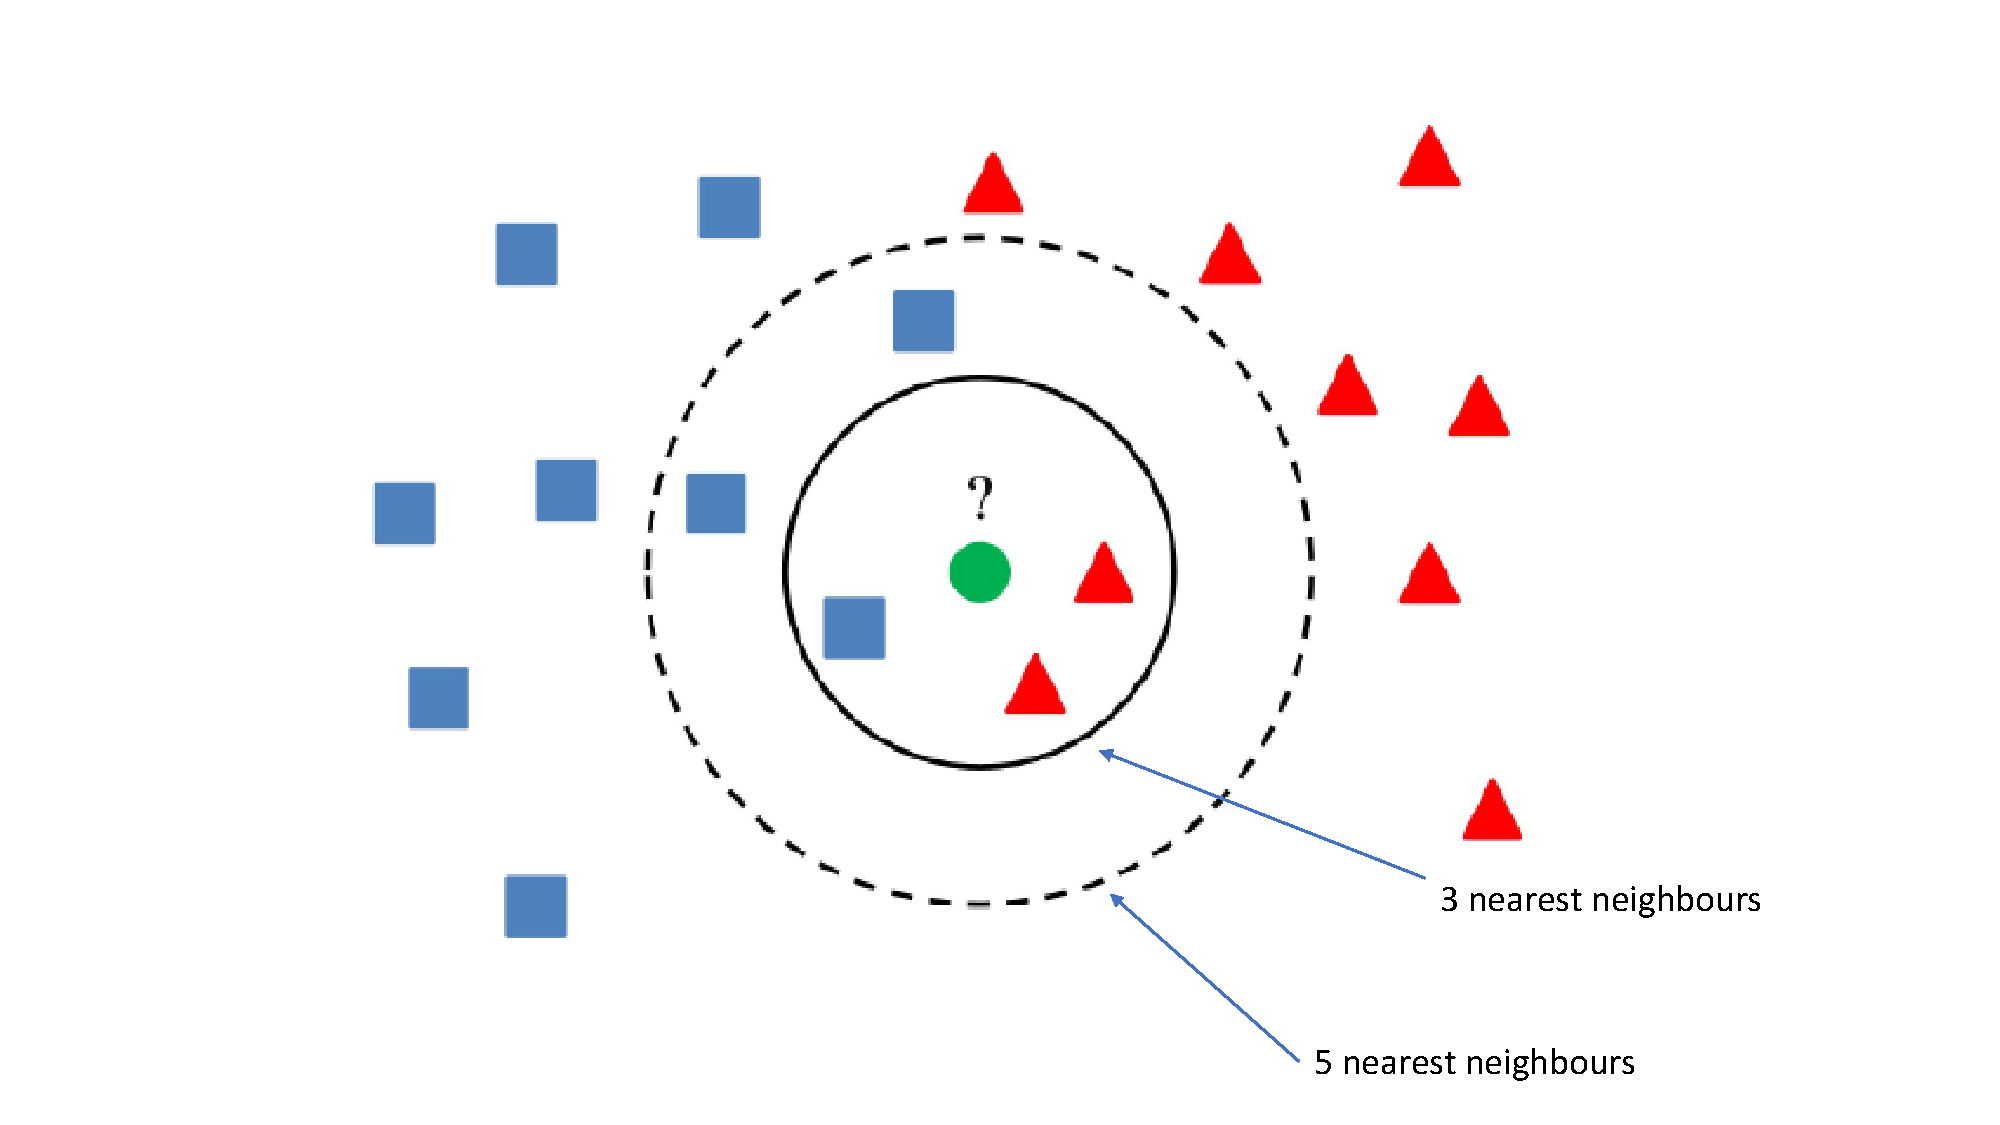
\includegraphics[width = 1\textwidth]{knn}

\end{frame}

\begin{frame}{How to choose $K$}
As we've seen different choice of $K$ can lead to different answers.
\begin{exampleblock}{Cross-validation}
	
	\begin{itemize}
		\item How to do we choose $K$ to minimise the test error
		\item We call $K$ a parameter
		\item We can apply a general method called cross-validation
		\item We split the training data (the data with labels) into random partitions
		\item Apply K-NN algorithm for different choices of $K$. E.g. $1,3,5,7,9,11$
		\item Compute the test error of each $K$
		\item repeat on different random partitions
		\item Choose the $K$ that minimises the average test error across random test partitions
		\item (Generally applicable method)
	\end{itemize}
 
\end{exampleblock}

\end{frame}

\begin{frame}{Cross Validation}
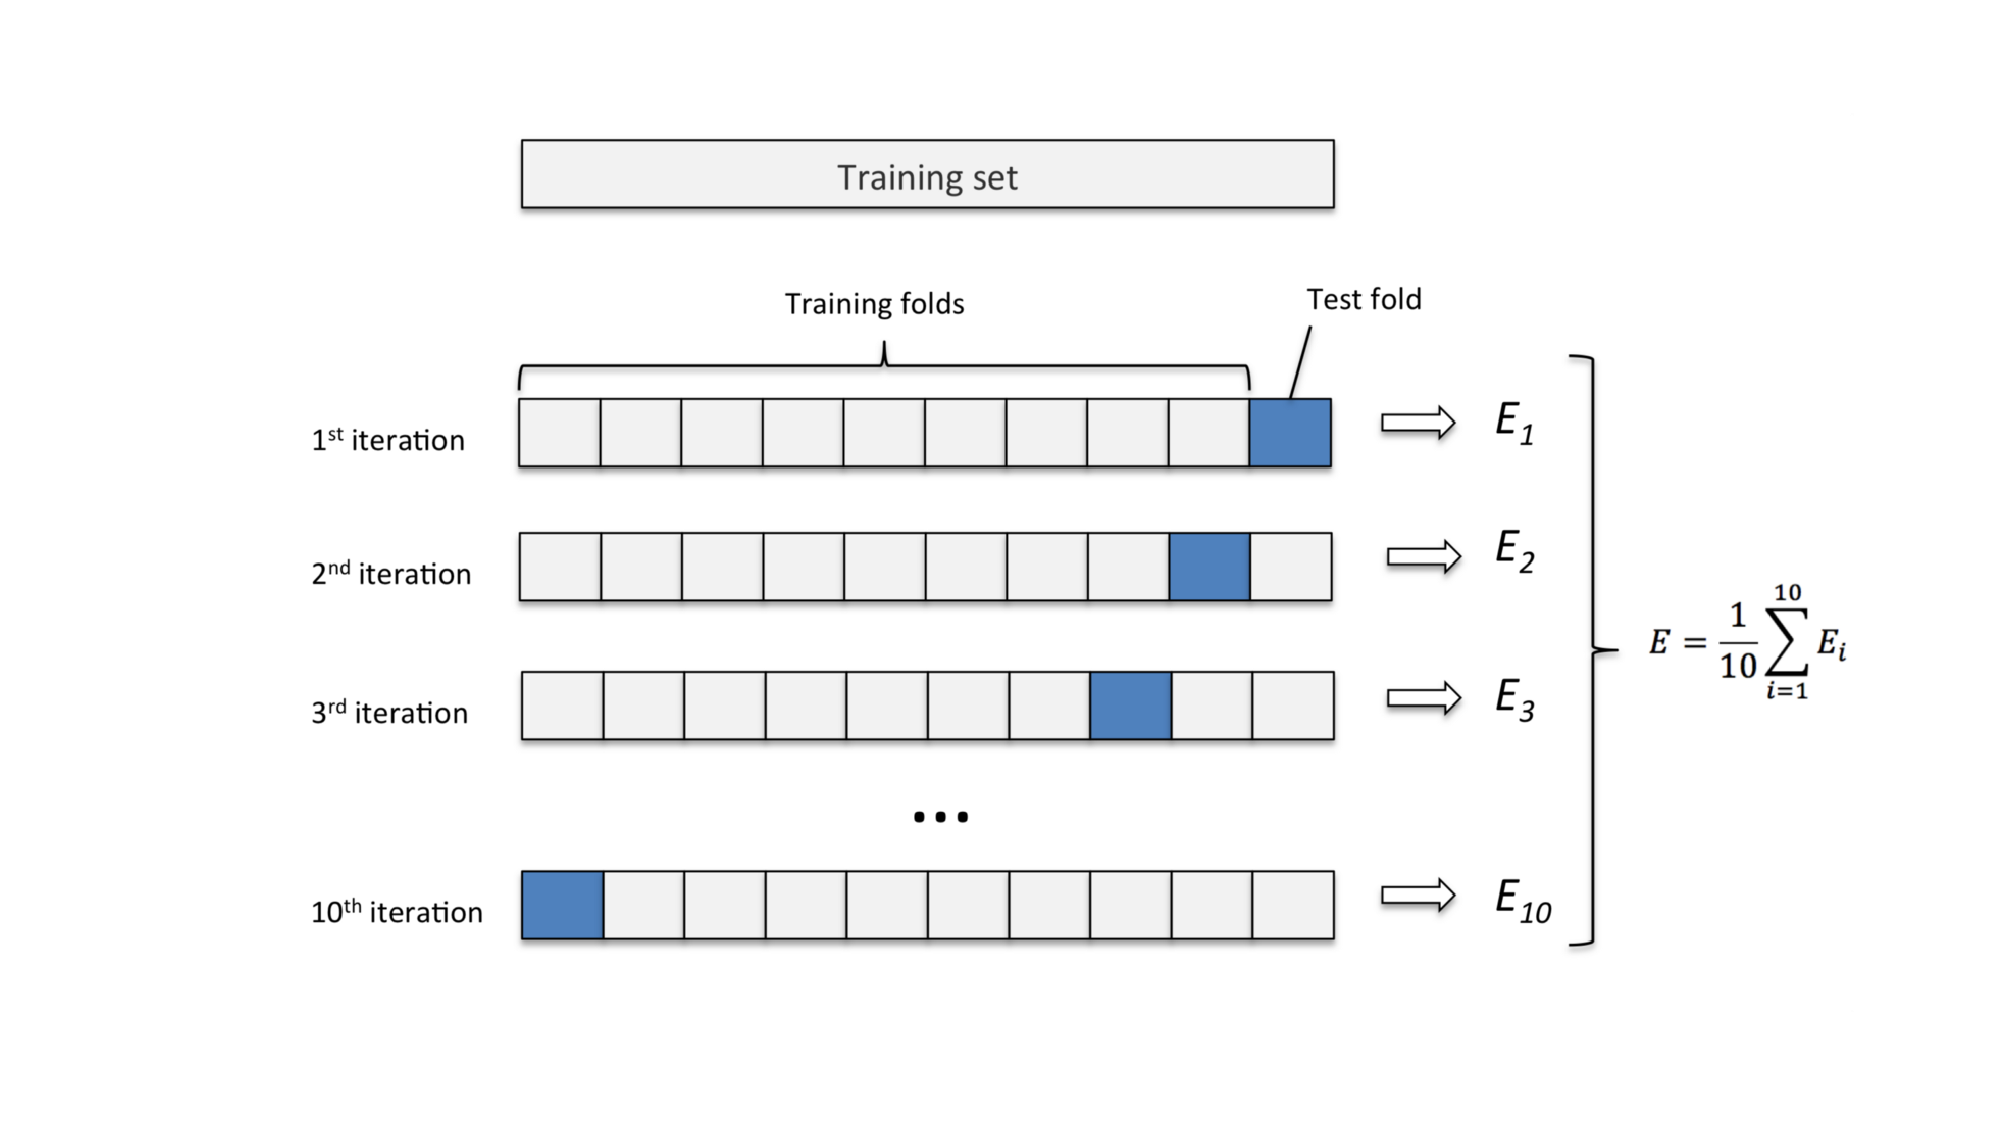
\includegraphics[width = 1\textwidth]{cv}
\end{frame}

\begin{frame}{Logistic Regression}

\begin{exampleblock}{Logistic Regression}
	
	\begin{itemize}
		\item The class output is related to a linear model
		\item Recall simple linear regression
		\begin{equation}
		y_i = \beta_0 + \beta_1x_i + \epsilon_i
		\end{equation}
		\item In logistic regression we want to model $P(Y = 1|X)$ a classification
		\item The logistic regression model makes the assumption that the log-odds are follow a linear model
		\begin{equation}
		\log\left(\frac{Pr(Y = 1|X)}{1 - Pr(Y = 1|X)}\right) = \beta_0 + \beta_1 X
		\end{equation}
		\item Regression coefficients are fitted with a method call maximum likelihood
		\item This is a general method for fitting model by maximising the probability of the model given the data.
	\end{itemize}
	
\end{exampleblock}

\end{frame}

\begin{frame}
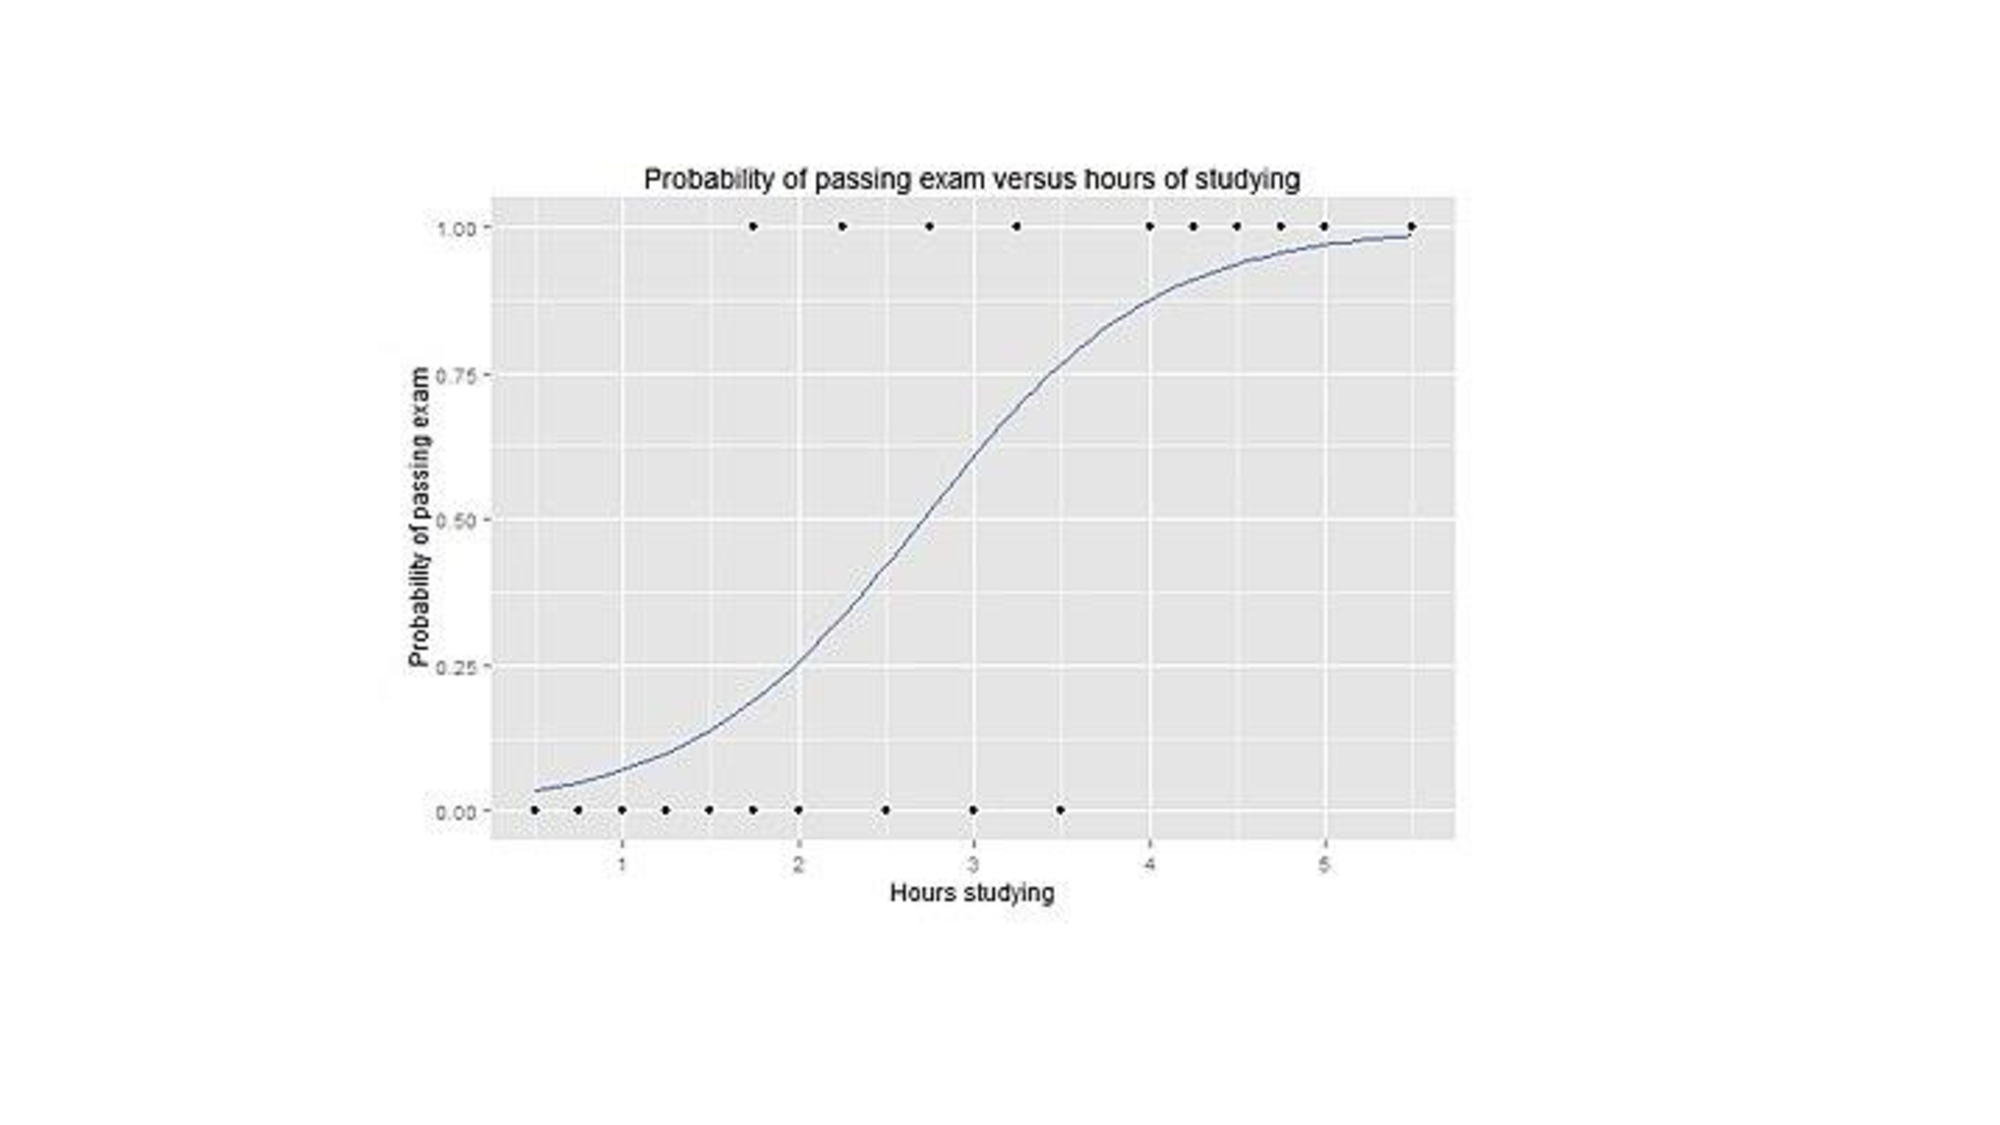
\includegraphics[width = 1\textwidth]{logistic}
\end{frame}



\begin{frame}{Is the variable useful for predicting the response?}

\begin{exampleblock}

\begin{itemize}
	\item We want a hypothesis test $H_0: \beta_1 = 0$
	\item Compute the $z$-statistic (which is normally distribution)
	\begin{equation}
	z = \frac{\hat{\beta}_1}{SE(\hat{\beta}_1)}
	\end{equation}
	\item Then compute p-values from the normal distribution
	\item Logistic regression can be extended in the same way as we say for linear regression
\end{itemize}

\end{exampleblock}

\end{frame}

\section{Clustering}

\begin{frame}{What is clustering}
\begin{exampleblock}{Aims and methods}
	
	\begin{itemize}
		\item We want to group data in a meaningful way
		\item We want to discover labels when we have no labelled data
		\item We want to partition data to make it easier to handle
		\item $K$-means
		\item hierarchical clustering
		\item spectral clustering (not covered)
		\item mixture models (not covered)
	\end{itemize}
\end{exampleblock}
\end{frame}

\begin{frame}{$K$-means}
	\begin{exampleblock}
		
		\begin{itemize}
		\item K-means is an iterative method
		\item We start with our data $X$
		\item We then select $K$ initial cluster centres
		\item Assign the points to the cluster with closest centre
		\item Compute a new centre for each cluster by computing the arithmetic mean of the points in each cluster
		\item Repeat until stability
		\item Answer will depend on initialisation so advised to repeat with random starting points
		\end{itemize}

	\end{exampleblock}

\end{frame}

\begin{frame}
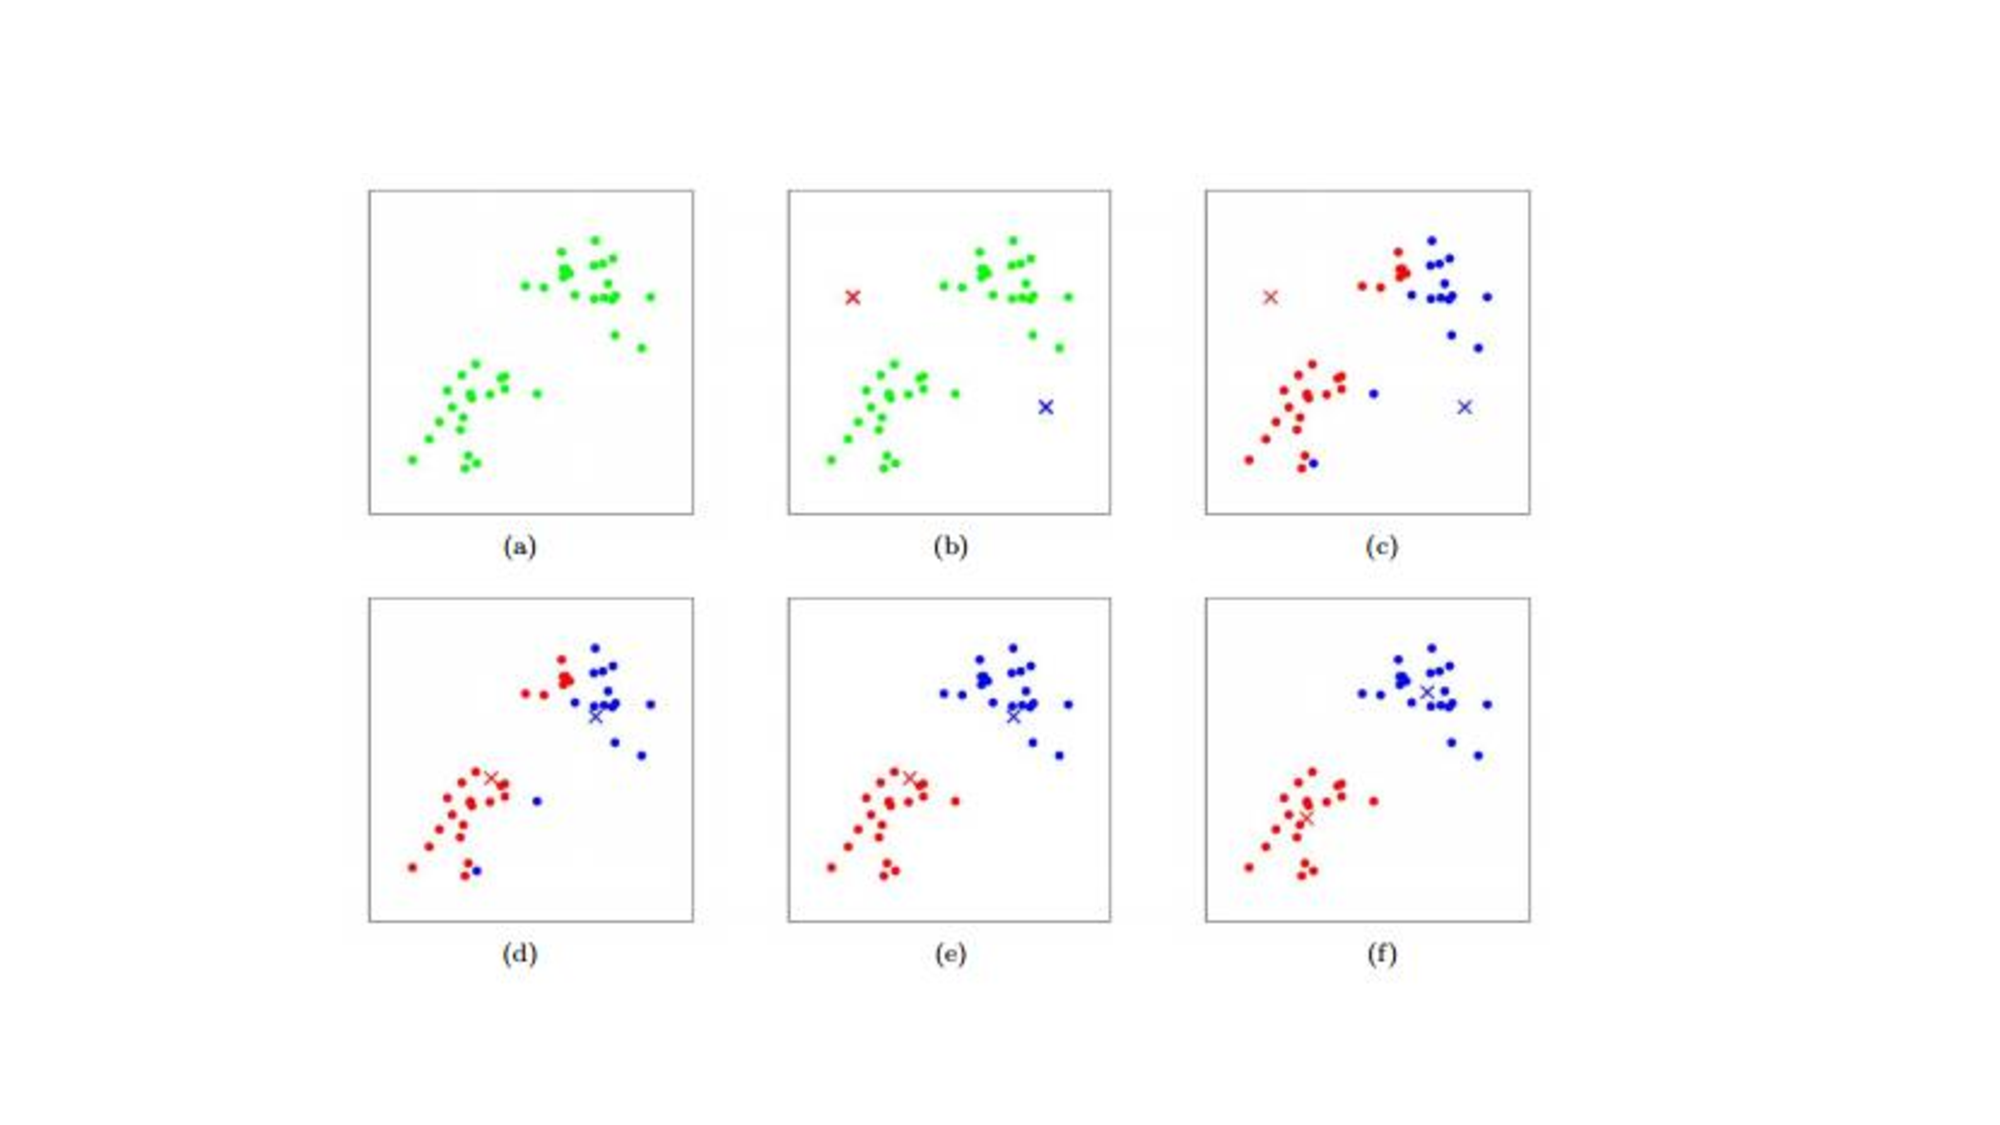
\includegraphics[width = 1\textwidth]{kmeans}
\end{frame}

\begin{frame}{How do we choose K?}
\begin{exampleblock}{Choosing K}
	\begin{itemize}
		\item Prior knowledge about the value of $K$
		\item Compute the Within Sum of Squares (WSS) for different values of $K$
		\item We can use the Elbow method; that is, look at where WSS beings to plateau and choose that $K$
		\item The Gap statistics (See MSMB)
		\item Other methods
	\end{itemize}
\end{exampleblock}
\end{frame}

\begin{frame}{Hierarchical clustering}
\begin{block}{Ideas}
	
\begin{itemize}
\item A bottom up approach
\item Start with by joining close "points" together (into a group)
\item As we work up we join groups of points together
\item Often visualised as a tree
\end{itemize}
\end{block}

\begin{exampleblock}{Distances}
	
	\begin{itemize}
\item single linkage computes the distance between clusters as the smallest distance between any two points in the two clusters
\begin{equation}
d_{12} = \min_{i \in C_1, j \in C_2} d_{ij}
\end{equation}
\item Complete linkage defines the distance between clusters as the largest distance between any two objects in the two clusters
\begin{equation}
d_{12} = \max_{i \in C_1, j \in C_2} d_{ij}
\end{equation}
\item Ward’s method minimize the variance within clusters.
\end{itemize}
\end{exampleblock}

\end{frame}



\begin{frame}{hierarchical clustering}

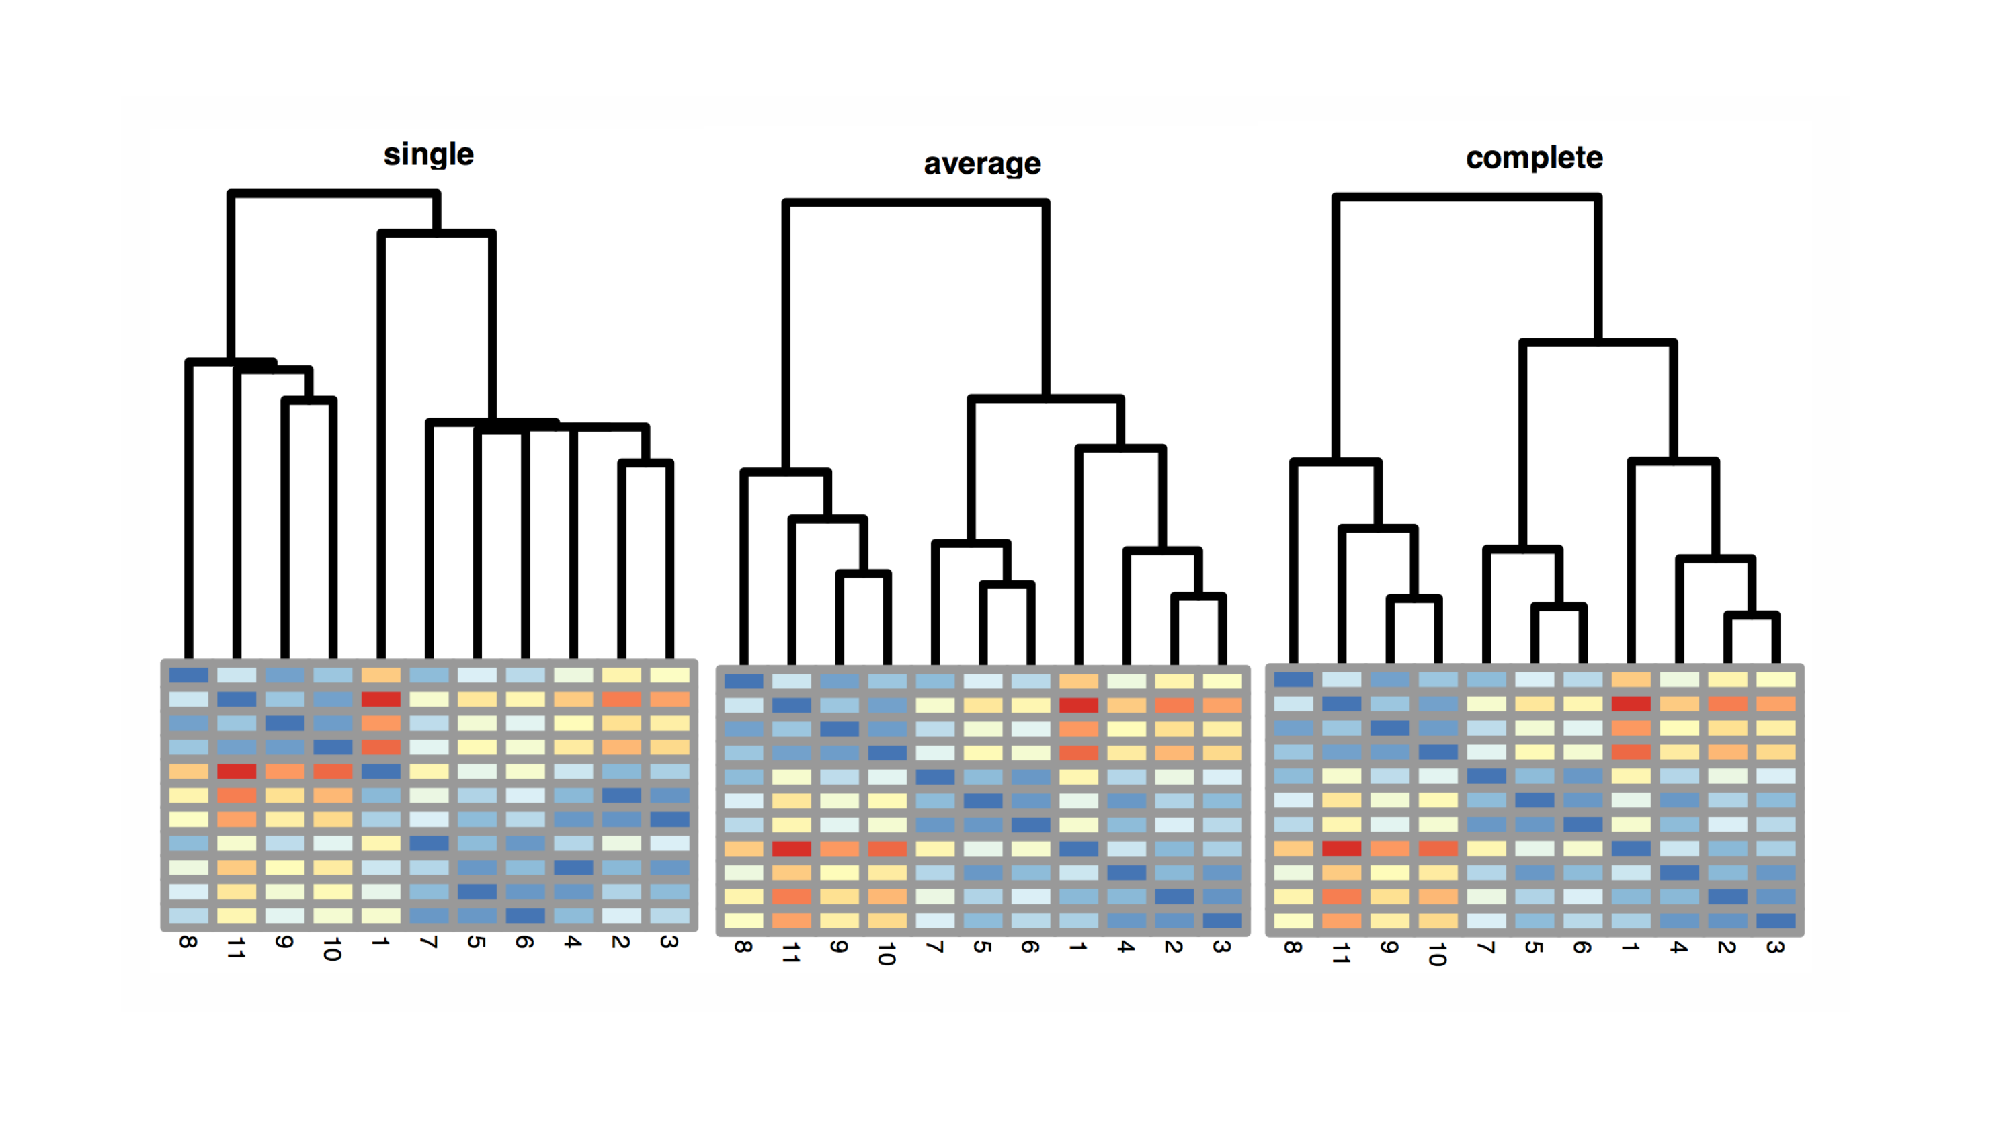
\includegraphics[width = 1\textwidth]{hclust}

\end{frame}

\begin{frame}{Summary}
\begin{exampleblock}{Summary}

\begin{itemize}
\item We discussed hypothesis tests including some example of tests
\item We covered different methods to deal with multiple testing
\item We discussed linear models and how to fit them
\item We discussed hypothesis tests for linear models and model fit
\item We covered multiple regression and regression with factors
\item We talked about PCA and CA
\item We discussed classification approaches such as KNN and logistic regression
\item We discussed clustering methods such as hierarchical clustering and K-means
\end{itemize}
\end{exampleblock}
\end{frame}

\begin{frame}{References}
Modern Statistics for Modern Biology; Susan Holmes and Wolfgang Huber
\\
An Introduction to Statistical Learning; James, Witten, Hastie, Tibshirnani
\\
The Elements to Statistical Learning; Friedman, Tibshirani, Hastie
\end{frame}


\end{document}